\documentclass[12pt, a4paper]{report}
\usepackage{a4wide}
\usepackage{anysize}
\usepackage[centertags]{amsmath}
\usepackage{amsfonts,amssymb,amsthm}
\usepackage{graphicx}
\usepackage{natbib}
\usepackage{wrapfig}
\usepackage{iitbieortitle}
\usepackage{pgf}
\usepackage{subcaption}
\usepackage{graphicx}
\usepackage{tocloft}
\usepackage[sorting=none]{biblatex}
\addbibresource{sample.bib}

%\usepackage{fullpage}
%\usepackage{rotating}
\usepackage{printlen}
\usepackage[ruled,vlined]{algorithm2e}
\usepackage{amsmath}
\usepackage{tikz}           % Package for 
\usepackage{algorithm}
\usepackage{subcaption}
\renewcommand{\baselinestretch}{1.2} %line spacing
\marginsize{1.2in}{1.2in}{1in}{1in}   %left right top bottom
\textwidth 6in
\setcounter{secnumdepth}{4}
% Title Page
%\bibliographystyle{unsrt}
\usepackage{hyperref}
%\usepackage[colorlinks=true,linkcolor=blue]{hyperref}%
\begin{document}



\pagenumbering{roman}
\pagestyle{plain}
\def\title{Microstructure Statistics}
\def\what{Dual Degree Project}
\def\who{Iyer Adithya Jairam (16D110011)}
\def\guide{Prof. M P Gururajan and Prof. Hina Gokhale}


\newcommand{\listequationsname}{List of Equations}
\newlistof{myequations}{equ}{\listequationsname}
\newcommand{\myequations}[1]{%
\addcontentsline{equ}{myequations}{\protect\numberline{\theequation}#1}\par}

\titlpage
\tableofcontents
\clearpage
\listoffigures
\clearpage
\listofmyequations

\newpage
\pagenumbering{arabic}

\chapter{Introduction}


% Write after everything else done

\chapter{Literature Survey}

Process-Structure-Property(PSP) relations have been an emerging field of study in the last decade, with significant advances in the domains of material characterization. Structure-Property relations, in particular have been extensively studied to accelerate the process of high throughput Computational Material design \cite{19kalidindi2016vision}. The idea behind this process is that, once we have sufficient databases of microstructure or other material characteristics, the process of developing new materials can be made faster by using the links in the Structure-Property relations. That is,we can predict the properties of new materials just by an interpolation of existing feature data of already processed materials. Furthermore, these relations can also provide us important insights into why certain features seen in the materials lead to distinct properties. 

Structure property relations are built upon the foundation of identifying the most important features from experimental tests on materials. For instance, in the microstructure itself, its phases and their spatial distribution often govern how they respond to external stress or stimuli, and a mapping from this spatial information to the property would fast-forward the selection of materials. The key to develop these relations is to have a robust method of extraction of useful features which capture most of the information associated with the material and has clear implications on the properties associated with it. In microstructures, the most common metric to judge the usefulness of these features is their ability to capture statistical and geometric spatial information, all the while being sufficient enough to enable reconstruction of the original microstructure or ensembles of it. Ensembles here refer to 2 microstructures of the same material, which might differ due to difference in observation time or location. The reconstruction of the original microstructure or ensembles of it would collate all microstructures of a material into a single class, thereby making the material accessible and easier to identify \cite{4fullwood2008microstructure}\cite{19kalidindi2016vision}.Reconstruction methods are also of importance, and efficiency of these methods is an improving field of study.

Once the features have been extracted, building structure-property relations involves training models on available experimental or simulated property data. A wide variety of methods to build these models have been suggested, and these have only picked up in number with the emergence of Machine Learning and their improved performance on classification and regression tasks \cite{18huang2020practicing}. The applications of these models are diverse, and shall be elaborated in further sections. 

The subsequent sections discuss the type of features and the methods to extract them, followed by reconstruction methods for 2D microstructures. This will be followed by discussion on feature compression and building models for structure-property relations. Microstructure evolution is another topic touched upon, and the methods in image processing dissected. Finally, the last section touches upon the recent push into Neural Networks and their implications.

\section{Spatial Features}

Spatial features or characterisation of microstructure must capture both geometric and statistical information. Geometric features generally consist of parameters related to shape and size of the local states. Local states can be defined as the phases of our microstructure at a point in space. Statistical features capture features like size distribution of the local states, probability of finding local states in space and alignment or anisotropy associated with the microstructure. In literature, the statistical parameters most frequently studied are the n-point correlation functions and linear path function.

\subsection{N-point correlation function}
The N-point correlation function is defined as finding 'n' specific local states in a local neighbourhood. In practice, the 2-point correlation function is much more ubiquitous. It can be defined as the probability of finding 2 specific local states at a spatial vector r from each other.
In isotropic microstructures, since the spatial distribution is direction invariant, a more common representation is in terms of $S_2^i(r)$, where $i$ represents the $i^{th}$ local state, r represents the distance and $S_2^i(r)$ is a function denoting the probability of finding 2 $i$ local states at a distance r from each other. 

Calculating $S_2^i(r)$ can be done most efficiently through Fast Fourier Transform methods \cite{12fullwood2008gradient}. Here, we can use the Convolution theorem in the Fourier space to simplify computation. Averaging across directions after calculating 2 point correlation presents us with the $S_2^i(r)$. $S_2^i(r)$ can also be calculated through Supervised Learning[20] as well.

2 Point correlations are efficient since they capture significant information about the sizes of the local states and their distribution in space. They also include information about the volume fraction of the 2 phases or local states. Visualization of the 2-point correlation function can capture both the anisotropy and sizes of individual local states. $S_2^i(r)$ can be considered as the 2-point correlation function averaged over all directions. $S_2^i(r)$ can give us information about the average distribution of states, but loses out on parameters representing anisotropy.

The correlations are particularly effective because they provide information to enable reconstruction of the original microstructures from the derived correlation function. Furthermore, for piece-wise uniform structures with smooth boundaries, the original microstructure can be completely reconstructed from only the 2-point correlation function\cite{5rozman2002uniqueness}, subject to a translation in space. This phenomenon is further demonstrated in \cite{4fullwood2008microstructure} for simulated microstructures. For ensembles of similar microstructure, the 2-point correlations show sufficient similarity to be considered as acquisition invariant features, and are extensively used in characterisation.

\subsection{Linear Path Function}
The Linear Path Functions captures the amount of clustering in a specific local state in the microstructures. It can be defined as the probability that a randomly oriented line segment of length r is completely encapsulated by a single phase\cite{21lu1992lineal}, say phase 1. Since the size of a phase is limited, the Linear path function, ie. $L_{11}(r)$, tends to 0 as $r$ increases. $L_{11}(r)$ is typically calculated by using Monte Carlo simulations, for both 2D and 3D microstructures.

The Linear Path function can also have the angle of inclination of the line segments $\theta$ and $\phi$ as a parameters for 3D microstructures, the function thus becomes $L_{11}(r,\theta,\phi)$ and $L_{22}(r,\theta,\phi)$ for the phases 1 and 2 respectively. Both these functions add information about anisotropy, and would converge to $L_{11}(r)$ and $L_{22}(r)$ for isotropic microstructures.

Calculation of these generally involves Monte Carlo simulations. In \cite{15singh2008image}, a method is presented where $L_{11}(r)$ can be calculated by moving a 1D array across an image, an counting the number of phase interfaces. Considering isotropic microstructures, this can be only done along the horizontal and vertical directions to calculate samples for $L_{11}(r)$ probability.

\subsection{Geometric and Further statistical Parameters}
In addition to the probability based descriptors, geometric features can add another layer of information. Traditional features of such kind provide information along 3 domains- 
\begin{enumerate}
    \item Composition : Described by the volume fraction of the phases
    \item Dispersion :  By calculating distances between precipitate centres 
    \item Size and Geometry: Calculated my measuring precipitate area and inclination
\end{enumerate}

Distributions of dispersion-length, size and geometry can be calculated, usually as normal distributions. Descriptions based on these parameters have also proved effective in characterization and reconstruction of the original microstructure \cite{16xu2014descriptor}. Furthermore, reconstruction of 3D microstructures from 2D image acquisitions have also proved successful, where 3D size and geometric parameters can be calculated by geometric operations on the 2D features \cite{17xu2014descriptor2}.

Since experimental data is often noisy, it requires digital pre-processing before being used to generate these features. This process generally takes place through binarization of the grey scale image after smoothing through Gaussian kernels. These binary images are mapped onto the original image to increase clarity and aid clustering. This is generally followed by identifying individual clusters and their centres to calculate the dispersion, size and geometry \cite{16xu2014descriptor}. 

\section{Reconstruction Methods}
The ability to reconstruct the original microstructure from the features is a metric to judge the quality of the features. Reconstruction methods traditionally involve a few basic common steps:

\begin{enumerate}
    \item Generate a sample reconstruction.
    \item Calculate feature vector from generated sample reconstruction.
    \item Compare sample feature vector with original image feature vector through a cost function.
    \item Exchange pixels in the sample such that the cost function is reduced, and report the image with a sufficiently low cost.
\end{enumerate}

Gradient based methods to calculate the pixel exchanges or modifications based on cost function do not work with such problems well \cite{12fullwood2008gradient}. The most common method followed in reconstruction is The\textbf{ Yeong and Torquato (YT) reconstruction method} \cite{13yeong1998reconstructing}. The YT Reconstruction method is studied further. 

\subsection{The Yeong and Torquato (YT) reconstruction method}
The primary reason the YT method is used is because of the presence of multiple local minima in the cost function. The YT method, also commonly referred to as \textit{simulated annealing} solves these issues. The YT method can be understood in the following steps \cite{3bostanabad2018computational}:

Let us define a cost function based on the original features $\hat{f_j}(r)$  and the model features $f_j(r)$ (from our generated model) as follows:
\begin{equation}
E = \sum_{j=1}^{m}\sum_{r=0}^{l}|\hat{f_j}(r)-f_j(r)|^2
\end{equation}
\myequations{Yeung Torquato cost function}

Here $r$ represents the various length scales, while $j$ iterates over the different statistical parameters(eg. 2-point correlation, Linear path function etc.)

Then, the YT method works as follows:

\begin{enumerate}
    \item Create an noisy sample image with the same volume fraction as the original image
    \item Calculate $f_j(r)$ from sample image, calculate E based on this $f_j(r)$ and $\hat{f_j}(r)$
    \item Swap pixels in image and recalculate E(call it $E_{new}$)
    \item If $E_{new} < E$,accept the swap. If $E_{new} > E$, accept it with a probability of $exp(-\frac{E_{new}-E}{T(k)})$, where $T(k)$ is defined as the Temperature at iteration $k$. $T$ is chosen such that the Bernoulli random variable of pixel exchange acceptance has a probability of 0.5 at k=0(ie. first iteration) \cite{13yeong1998reconstructing}.
\end{enumerate}

The $4^{th}$ step is crucial to escape the local minima, and converge to the global minima for the reconstruction. The YT method is computationally expensive, and other methods like sequential quadratic programming methods \cite{12fullwood2008gradient} or Markov Random Fields \cite{8liu2015random} have also been used for reconstruction.

\section{Building structure-property relations}

Once the characterisation is complete and the features hold sufficient information about the microstructure, models can be built to map structure to properties. Since the features are often large in number, it is often reduced in size by linear combination of features through methods like Principal Component Analysis.

The process can be defined as follows:

\begin{enumerate}
    \item Generate ensemble of microstructures and derive selected features from each microstructure.
    \item Represent condensed microstructure features as the components of the features onto the principal axis.
\end{enumerate}

It has been observed that the first 3 principal components can account for over 80\% of the variance in the features \cite{9paulson2017reduced}. Once this reduced order feature set is available, it can be used for purposes like clustering or classification of microstructures based on distances between the components[6]. Clustering algorithms like K-means clustering can be utilized for this clustering. Furthermore, components can also be used to predict bulk properties like Young's modulus by using linear regression \cite{9paulson2017reduced}. Thus, this reduced order representation can simplify and speed up training in the supervised learning processes. The one drawback with PCA is that the principal components are often large in size and do not signal any physical or intuitive meaning, making them a mathematical operation.

Process-structure relations can also be predicted on the basis of components of feature vectors. For instance given a training set of temperature, aging time and microstructure of a sample, a classification model has been shown to predict the process parameters from a test set \cite{2yabansu2019application}. Thus, the flexibility of using feature vectors with supervised learning techniques gives us many avenues to tackle in the Process-Structure-Property domain.

\section{Microstructure Evolution}

Aside from deriving structure property relations and reconstruction of the microstructure, features derived can be used to study the evolution of the microstructure in time. Tracking the features as a function of time gives us important information about the evolution process like rate of phase separation, precipitate growth and agglomeration. Furthermore, effect of process on structure can be quantified through these features and thus process fine-tuning or adjusting can be improved. 

Tracking the growth of a particular particle can explain particle kinetics, as explained in \cite{10roosen1998simulations}. It is observed that precipitate growth is rapid in the initial stages of growth due to the diffusion of solute from the matrix phase. It is in this region that the phase separation is rapid, and the growth plateaus henceforth. That is, at this point in time all neighbouring phase has been absorbed into the.precipitate. \textbf{Roosen et al}.\cite{10roosen1998simulations} also show that the precipitate approaches it's Wolff shape as evolution continues. Furthermore, the elongation and inclination of the precipitate has been observed to increase in time using precipitate tracking techniques. 

Multi-particle statistics have also been studied wherein the average size of the precipitates is tracked. The steep ascent in the average size of the precipitates is observed as expected. Shrinking of smaller particles leading to disappearance and agglomeration can also be observed through precipitate tracking techniques \cite{10roosen1998simulations}.

Aside from growth tracking of precipitates, interface velocity has also been of interest specially in simulated microstructure. Since the microstructures are represented as composition values in discrete spatial locations represented by pixels in an image, the discontinuity and non-differentiable nature of images is a challenge in calculating velocity. The sudden drop in composition in the phase interface rule out computational methods of calculating velocity since they involve numerically calculating the gradients. Thus, to be able to find the gradient at values in the image, the image needs to be smoothed by functions. The most common method of smoothing is by using Gaussian kernels. Other methods are also suggested like using a smoothed sign function \cite{22park2014application}, which deals with 2 specific problems of Gaussian kernels. Firstly, the location shift of the interface due to Gaussian smoothing is corrected, and the curvatures are more appropriately defined by using the smoothed sign function. Other methods like diffusion smoothing are also applied as mechanisms to improve calculation of gradients . 

Once the image is smooth, Level Set Methods can be applied to calculate parameters like velocity, inclination and curvature \cite{23sethian1999level}. Level set methods are numerical computations which can be used to calculate the movement of the interface, based on gradients. For level set methods to be useful, the image needs to be transformed to it's Signed Distance Function(\textbf{SDF}), where locations inside the interface have a value $>$ 1, outside $<$ 1 and the interface needs to have a value of 0. Level Set methods can also be easily extended to calculate 3D interface properties \cite{22park2014application} like mean curvature, Gaussian curvature and normal velocity.

Applications of particle tracking are diverse, and it is a commonly studied phenomenon in fields like biology and earth science. Applications in material sciences can be seen in study of sintering using phase transformation \cite{1biswas2018phase} and in the modelling of battery separators \cite{11xu2019stochastic}.

\section{Deep Learning}

Recent advances in Deep learning with the advent of Convolutional Neural Networks \cite{24lecun2015deep} and GPUs have accelerated the utilization of deep non-linear classifiers. Deep learning has been utilized to find low dimensional features from image ensembles to complement the 2-point correlations functions \cite{25lubbers2017inferring}. Deep neural networks have also been used to relate microstructure to the susceptibility to damage initiation \cite{26venkatraman2020reduced}. Deep learning could be tremendously useful in the modelling of structure property relationships as well as generation microstructure ensembles. The availability of large amounts of data is what makes neural networks particularly effective, and with the increasing focus on material database creation, it is likely to be crucial.


















\chapter{Methodology and Formulation
}
\section{Data Description and Pre-processing}

\subsection{Data Description}
The data generated is in the form of .dat files, with each .dat file representing one microstructural image. Each image consists of $2048* 2048$ pixels, with each pixel representing the composition at a spatial location, ie. the pixel values ranged between 0 and 1. The pixels with values $>=0.5$ are considered as precipitates in our analysis.

The generated microstructure for $200000$ time steps is sampled after every $100$ time steps, thus the total number of images obtained are $2000$. For some cases, sampling after every 200 time steps produced 1000 images. In such cases, analysis is done on $1000$ images with each image having a resolution of $2048*2048$. Three sets each of Cahn-Hilliard circular microstructures and hexagonal microstructures are generated, with the compositions for the minor component set at $0.3$, $0.4$ and $0.5$ for each respectively.


\subsection{Data Pre-processing}
Statistical analysis of shape, size and distribution often requires the image pixel values to be more differential for gradient calculations, and binary for image shape and size quantification. Thus these data pre-processing steps are essential to improve precision of the algorithms henceforth mentioned.

The images are first made continuous by convolution of the image with a $5*5$ Gaussian filter to remove shape discontinuities, and make the gradient($1st$ derivative) smooth. After smoothening, the microstructure was binarized by replacing pixel values $>=0.5$ by 1 and $<0.5$ by 0. This binary microstructure is henceforth used as the image for study.

\begin{figure}[H]
\centering
\begin{subfigure}{0.45\textwidth}
  \centering
  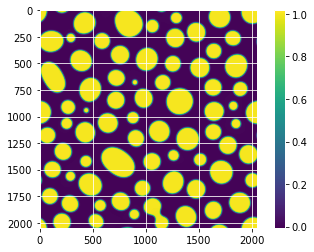
\includegraphics[width=0.9\textwidth]{Pictures/DataProcessingNonSmoothened.png}
  \caption{Raw microstructure Image}
  \label{img:microstrImg}
\end{subfigure}
\begin{subfigure}{.45\textwidth}
  \centering
  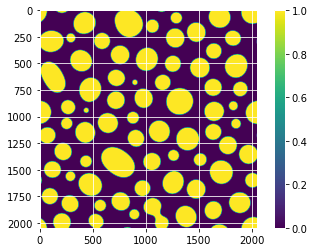
\includegraphics[width=0.9\textwidth]{Pictures/DataProcessingSmoothened.png}
  \caption{Smoothened and binarized image}
  \label{img:MicrostrImg}
\end{subfigure}
\caption{Visualizing data: The higher intensity of yellow in the binarized image corresponds to 1(perfectly yellow). The sharp phase boundaries are noticeable in (b)}.
\label{fig:test}
\end{figure}

%%%%%%%%%%%%%%%%%%%%%%%%%%%%%%%%%%%%%%%%%%

\section{2 Point Statistics}
\subsection{Formulation}
Quantifying the spatial distribution of states in a microstructure can help us capture the density of precipitate and define how isotropic or anisotropic a particular microstructure is. We calculate these distributions in terms of the microstructure probability function $m_s^n$, defined as the probability of finding the local state $n$ at the spatial location $s$. In our binary microstructures, the $m_s^n$ values are either $1$ or $0$, ie. a local state is either present or not present at a particular spatial location. 

We extend this formulation to include 2 local states, and define $f_t^{n_1n_2}$ as the probability of finding local state $n_1$ at a spatial location while simultaneously finding $n_2$ at a spatial location $t$ vector away from the original spatial location. This value can be calculated as follows \cite{4fullwood2008microstructure}:

\begin{equation}
f_t^{n_1n_2} = \frac{1}{S}\sum_{s=0}^{S-1} {m_s^{n_1}}{m_{s+t}^{n_2}}
\end{equation}
\myequations{2-Point Correlation}

We solve the above sum by taking the $LHS$ and the $RHS$ into the Fourier space and apply the Convolution theorem to the $RHS$ expression. This gives us the Fourier transform of $f_t^{n_1n_2}$ as:

\begin{equation}
F_k^{n_1n_2} =\mathfrak{F}(\sum_{s=0}^{S-1}{m_s^{n_1}}{m_{s+t}^{n_2}})= \frac{1}{S} \sum_{s=0}^{S-1}{m_s^{n_1}}{e^{\frac{-2{\pi}isk}{S}}}  \sum_{z=0}^{S-1}{m_z^{n_2}}{e^{\frac{2{\pi}izk}{S}}}
\end{equation}
\myequations{Fourier Space representation of 2-Point correlation}


We then take the inverse Fourier transform of the above expression to calculate the 2 point correlations. 

Here, if $n_1$ and $n_2$ are the same local state in our binary microstructures({1,1} or {0,0}), the $f_t^{n_1n_2}$ values would represent the \textbf{auto-correlations} of the local states 1 and 0 respectively. Alternatively, if $n_1$ and $n_2$ are the different local states, ie. ({1,0} or {0,1}), the $f_t^{n_1n_2}$ values would correspond to the \textbf{cross-correlation} of the 2 local states.

\subsection{Algorithm}
We utilize the python library $numpy$ to calculate the auto-correlation and cross-correlation values, since it supports swift calculation of Fourier and inverse-Fourier transform. The microstructure probability function $m_s^{n_i}$ is calculated for each of the $i^{th}$ local state, and stored as $numpy$ arrays mi(m1, m2 etc.). The flowchart below summarizes the process followed in calculating the correlations.

\usetikzlibrary{shapes.geometric, arrows}
\tikzstyle{process} = [rectangle, minimum width=3cm, minimum height=1cm, text centered, draw=black]
\tikzstyle{arrow} = [thick,->,>=stealth]
\begin{center}
\begin{tikzpicture}[node distance=2cm]
\node (start) [process] {Calculate m1 and m2};
\node (in1) [process, below of=start] {Fourier transform of m1 and m2(M1 and M2) };
\node (in2) [process, below of=in1] {Inverse Fourier Transform of M1*conjugate(M2)/(No of pixels)};
\node (in3) [process, below of=in2] {Absolute value, followed by reshaping(fftshift) to image size};
\draw [arrow] (start) -- (in1);
\draw [arrow] (in1) -- (in2);
\draw [arrow] (in2) -- (in3);
\end{tikzpicture}
\end{center}

\subsection{Visualization}
The probability correlation values are visualized by representing the probability values as colors of varying intensities, centred at the origin of the image. Since we take the Fourier and Inverse Fourier transform of the image, we use the \textit{fftshift} command so that all the zero frequency values are closer to the centre. Since we are visualizing vectors at all directions, looking at them with the zero vector at the centre of the image aids comprehension. Thus, they are centered at the origin. Once the correlations are captured, we can calculate the radial probability distribution, as well as the probability distributions at various angular sectors. These visualizations are presented below:

\begin{figure}[H]
\centering
\begin{subfigure}{.45\textwidth}
  \centering
  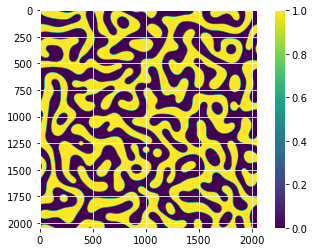
\includegraphics[width=0.9\textwidth]{Pictures/2 Point/2_point_binary_image.jpeg}
  \caption{Raw microstructure Image}
  \label{img:microstrImg}
\end{subfigure}
\begin{subfigure}{.45\textwidth}
  \centering
  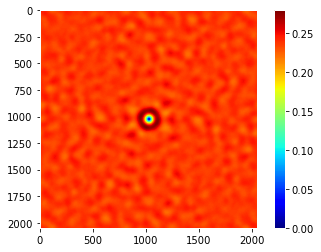
\includegraphics[width=0.9\textwidth]{Pictures/2 Point/2_point_stats_bw.jpeg}
  \caption{Cross Correlation}
  \label{img:microstrImg}
\end{subfigure}
\begin{subfigure}{.45\textwidth}
  \centering
  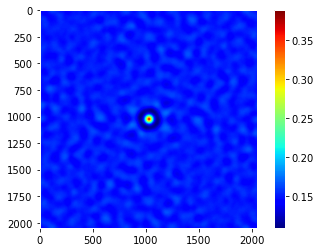
\includegraphics[width=0.9\textwidth]{Pictures/2 Point/2_point_stats_ww.jpeg}
  \caption{1-1 Auto-Correlation}
  \label{img:microstrImg}
\end{subfigure}
\begin{subfigure}{.45\textwidth}
  \centering
  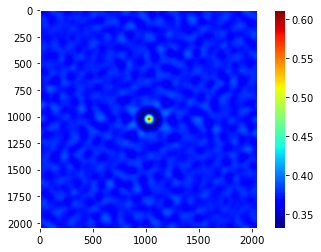
\includegraphics[width=0.9\textwidth]{Pictures/2 Point/2_point_stats_bb.jpeg}
  \caption{0-0 Auto-Correlation}
  \label{img:microstrImg}
\end{subfigure}
% \begin{subfigure}{.45\textwidth}
%   \centering
%   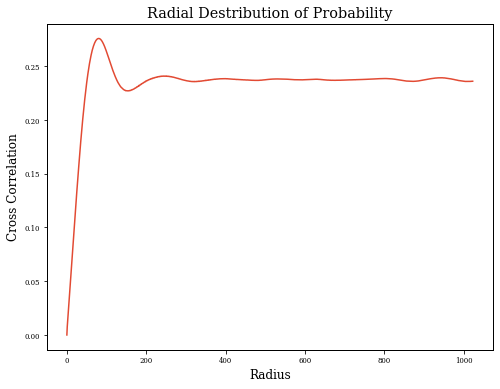
\includegraphics[width=0.9\textwidth]{Pictures/2 Point/2_point_stats_radial.jpeg}
%   \caption{Radial Cross Correlation}
%   \label{img:microstrImg}

% \end{subfigure}

\caption{Visualizing Correlations}
\label{fig:test}
\end{figure}

These visualizations and the probabilities were bench-marked against the \textit{PYMKS python library} \cite{27wheeler2014pymks}, where they gave identical results. 
%%%%%%%%%%%%%%%%%%%%%%%%%%%%%%%%%%%%%%%%%%%%%%

\section{Level Set Methods and Velocity Formulation}

Calculating velocity of interface is important since it gives us a good metric to judge pace of precipitate growth, and understand the inherent qualitative properties of the 2 phases. We have used the Level Set Method \cite{23sethian1999level} to quantify the orthogonal velocity at the interface of the 2 phases. Velocity studies are important because they let us visualize how a particular precipitate is growing, identify regions of rapid growth and distinguish between 2 similar looking microstructures.
 
\subsection{Level Set Methods: Formulation}
The problem statement can broadly be broken down into 3 parts, locating the interface, finding the normal to the interface to suggest direction of movement and finding the magnitude of the interface velocity. We study the 3 parts separately:

\subsubsection{Contouring or Interface Location}
We define the interface pixels as the pixels which have at least one bordering(vertical, horizontal or diagonal) precipitate pixel. Thus for a single pixel precipitate, we would have 8 bordering interface pixels. The presence of diagonally neighbouring points do not harm our calculations, since we smooth the binary image, and the gradients formed post smoothing are nearly equal in orthogonal and diagonal neighbours. The figure below illustrates the contours found for a hexagonal microstructure. Because the contours are fine, the image has to be zoomed in to notice the contours as computer rendering makes the faint lines more transparent.

\begin{figure}[H]
\centering
\begin{subfigure}{.6\textwidth}
  \centering
  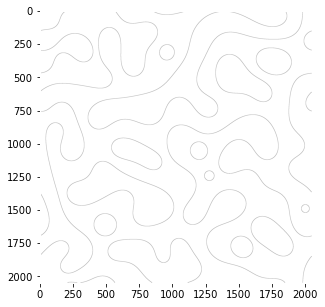
\includegraphics[width=0.9\textwidth]{Pictures/niceContours.png}
  \label{img:microstrImg}
\end{subfigure}
\caption{Contours on the microstructure}
\label{fig:test}
\end{figure}

\subsubsection{Interface direction and velocity}
The interfacial velocity and direction of a growing or shrinking precipitate can be captured by applying level set methods. This involves first converting the binary image into a continuous \textbf{signed difference function}($\Phi$). We do this by first smoothing the image by the convolution of a 5x5 Gaussian kernel on the image, and then subtracting 0.5 to make the interface pixels close to 0 to create the signed difference function($\Phi$).  

Once we have obtained the Signed Difference Function($\Phi$), we can apply Level Set Algorithms to find the interface normal vector and the velocity. The normal vector $\vec{N}$ and the velocity magnitude $|\vec{V}|$.

\begin{equation}
\vec{N} = -\frac{\nabla\Phi}{|\nabla\Phi|}
\end{equation}
\myequations{Level set normal vector}


\begin{equation}
|\vec{V}| = \frac{\frac{d\Phi}{dt}}{|\nabla\Phi|}
\end{equation}
\myequations{Level set velocity}


Here, the sign of $\frac{d\Phi}{dt}$ decides whether an interface is expanding or contracting. Furthermore, $\frac{d\Phi}{dt}$ was calculated by interpolating a line through 4 points, to make the derivatives more representative of the actual curve.

\subsection{Algorithm}

We followed the following process while calculating the interface velocities of the precipitates in our microstructures. 

\usetikzlibrary{shapes.geometric, arrows}

\tikzstyle{process} = [rectangle, minimum width=3cm, minimum height=1cm, text centered, draw=black]
\tikzstyle{arrow} = [thick,->,>=stealth]
\begin{center}
\begin{tikzpicture}[node distance=2cm]
\node (start) [process] {Find interface pixels};
\node (in1) [process, below of=start] {Calculate Signed Difference Function $\Phi$};
\node (in2) [process, below of=in1] {Calculate interface normal vector($\vec{N}$) and velocity magnitude($|\vec{V}|$)};
\node (in3) [process, below of=in2] {Multiply $\vec{N}$ and $|\vec{V}|$ to get velocity vector};
\node (in4) [process, below of=in3] {Plot quiver plot of velocity vectors by selectively selecting points};
\draw [arrow] (start) -- (in1);
\draw [arrow] (in1) -- (in2);
\draw [arrow] (in2) -- (in3);
\draw [arrow] (in3) -- (in4);
\end{tikzpicture}
\end{center}


\subsection{Visualization}
Since we are working with large size images, plotting the quiver plot by considering each interface pixel would inundate the figure with arrows. Furthermore, the nearby boundary pixels do not show significant deviation in velocity vectors. Thus we plot only every $8^{th}$ velocity vector for better visualization. 

The algorithm is tested on a continuously growing perfectly spherical microstructure, whose growth rate is calculated geometrically and validated.

\begin{figure}[H]
\centering
\begin{subfigure}{.6\textwidth}
  \centering
  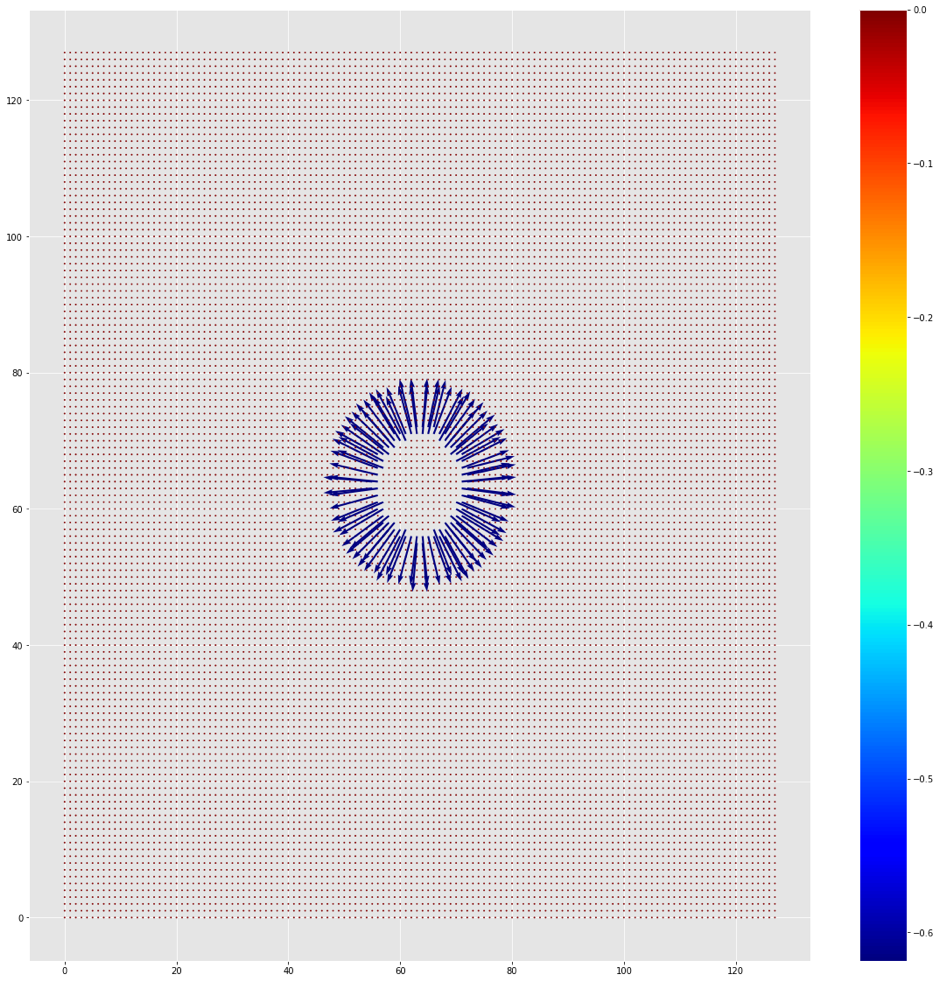
\includegraphics[width=0.9\textwidth]{Pictures/Level Set/level_set_velocity.png}
  \label{img:microstrImg}
\end{subfigure}
\caption{Velocity visualized on a quiver plot}
\label{fig:test}
\end{figure}

% %%%%%%%%%%%%%%%%%%%%%%%%%%%%%%%%%%%%%%

\section{Hoshen-Kopelman Algorithm and Application}

\subsection{Formulation: General Hoshen-Kopelman}

The general Hoshen-Kopelman \cite{28hoshen1976percolation} is one of the most efficient algorithms for cluster counting and labelling since it takes only one pass through the image to label the clusters in the image. We take a sample binary microstructure image and apply the regular Hoshen-Kopelman algorithm, which does not account for periodic boundary conditions to test our algorithm for Non-periodic images. The general algorithm without PBC is implemented as follows \cite{29fricke2004hoshen}, without considering the boundary pixels:

\begin{algorithm}[H]
\SetAlgoLined
\KwResult{A matrix of labels}
 maxlabel=0\;
 \For{x in 0:no of columns and y in 0:no of rows}{

   \If{occupied[x,y]}{
   left = occupied[x-1,y]\;
   above = occupied[x,y-1]\;
    
    \If{left != 0 and above == 0}{
     label[x,y] = find(left)\;}
    \If{left == 0 and above != 0}{
     label[x,y] = find(above)\;}
    \If{left == 1 and above == 1}{
     union(left,above), \;
     label[x,y] = find(left)\;}
     
     }
   }
 \caption{Hoshen Kopleman algorithm for Non-PBC}
\end{algorithm}

Here, the union and find methods are derived from the common union-find algorithm. The union find algorithm is one of the most intensively studied and analyzed algorithms in the world, and the \textbf{Weighted Union Find with Path Compression} technique is implemented to optimize the efficiency of the algorithm. The technique is useful as it can shorten the trees which are formed in the union find algorithms and also account for complexity in the nodes which are formed.

The Hoshen-Kopelman algorithm works well for non-periodic boundary conditions, but requires modifications for periodic boundary conditions. The specific problem with periodic boundary conditions is that the edge pixels could belong to the same cluster, and thus the above algorithm fails.

\subsection{Formulation : Hoshen Kopleman for PBC}
To account for periodic boundary conditions, we follow the original Hoshen-Kopelman algorithm to completion. Post completion, we run the algorithm again only on the edge labels/pixels with two key changes:

\begin{enumerate}
    \item We do not allot a new label value to a cluster encountered for the first time, instead we let it retain the earlier label
    \item We introduce the periodic boundary condition to the $1^{st}$ row and column of the image by defining it's left and above boundary pixel by adding a imaginary row and column to the left and top of the image. 
\end{enumerate}

The algorithm for periodic boundary conditions is as follows:

\begin{algorithm}[H]
\SetAlgoLined
\KwResult{A matrix of labels}
 maxlabel=0\;
 \For{x in 0:no of columns and y in 0:no of rows}{

  \If{occupied[x,y]}{
  left = occupied[x-1,y], \;
  above = occupied[x,y-1]\;
    
    \If{left != 0 and above == 0}{
     label[x,y] = find(left)\;}
    \If{left == 0 and above != 0}{
     label[x,y] = find(above)\;}
    \If{left == 1 and above == 1}{
     union(left,above), \;
     label[x,y] = find(left)\;}
    \If{left == 0 and above == 0}{
     maxlabel=maxlabel+1, \;
     label[x,y] = maxlabel\;}
     }
  }
  \For{x in 0:no of columns and y in 0:n0 of rows}{

  \If{occupied[x,y] and edge[x,y]}{
  left = occupied[x-1,y] (PBC), \;
  above = occupied[x,y-1] (PBC)\;
  
    \If{left != 0 and above == 0}{
     label[x,y] = find(left)\;}
    \If{left == 0 and above != 0}{
     label[x,y] = find(above)\;}
    \If{left == 1 and above == 1}{
     union(left,above), \;
     label[x,y] = find(left)\;}
     }
  }
 \caption{Hoshen Kopleman algorithm for PBC}
\end{algorithm}

\subsection{Visualization}
We visualize the cluster labelled microstructure by color coding each precipitate based on its number. We can also visualize a single precipitate by projecting only one label. In Figure \ref{fig:hoshKopExImg}, each precipitate is uniquely represented by a colour, whose numerical value can be found by using the colour-bar. The colour-bar also gives us information like the total number of precipitates, which in Figure \ref{fig:hoshKopExImg} are around $225$. This figure will henceforth be called as the Hoshen-Kopelman Labelled Microstructure(HSLM) image of a microstructure.

\begin{figure}[H]
\centering
\begin{subfigure}{.6\textwidth}
  \centering
  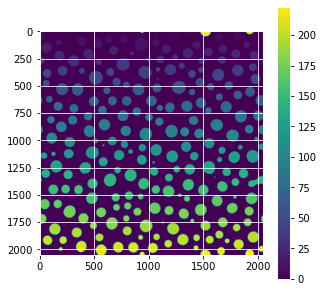
\includegraphics[width=0.9\textwidth]{Pictures/Hoshen/Hoshen_kopleman.jpeg}
\end{subfigure}
\caption{Cluster counting and labelling(HKLM Image)}
\label{fig:hoshKopExImg}
\end{figure}


%%%%%%%%%%%%%%%%%%%%%%%%%%%%%%%%%%%%%%%%%%%%%%

\section{Shape/size quantification and Precipitate Tracking}

\subsection{Shape/size quantification}
Identifying features of precipitates like size, inclination etc can help us study precipitate growth and evolution in detail. Once we have identified a precipitate(by using the Hoshen-Kopelman algorithm), we can derive many features of the precipitate by analyzing the binary microstructure of the precipitate.

The two main proponents which are required to track and study a precipitate are the centre of gravity and the $2^{nd}$ order moment of the binary shape. The centre of gravity is associated with the spatial position of the precipitate and the moment is associated with the shape/inclination of the image. What makes it challenging is to extend the usually simplistic analysis on generic binary images to images with periodic boundary conditions. We will investigate the 2 problems separately in this section.

\subsubsection{Centre of gravity}
Centre of gravity for generic non-periodic binary images is directly obtained by orthogonal counting of precipitate pixels in both directions, and then finding the weighted mean of the resulting array. Since we are working with periodic boundary conditions, we first move from a linear array to an angular array, and do the weighted means in the rotational space \cite{30bai2008calculating}. The physical equivalent of our approach would be folding the image to calculate the COG. The algorithm for one direction, say x, is described as follows. Given a directional array $x_i$ going from 1 to X and a weight distribution $m_i$ which adds up to $M$:

$$
\theta_i = \frac{2{\pi}x_i}{X}
$$

$$
\alpha_i = \cos{{\theta}_i}
$$

$$
\beta_i = \sin{{\theta}_i}
$$

$$
\Bar{\alpha_i} = \frac{1}{M}\sum_i {m_i}{\alpha_i}     
$$

$$
\Bar{\beta_i} = \frac{1}{M}\sum_i {m_i}{\beta_i}
$$

$$
\Bar{\theta} = arctan(-\Bar{\beta_i},\Bar{\alpha_i})+\pi
$$

\begin{equation}
    X_{cog} =\frac{X{\Bar{\theta}}}{2\pi}
    \label{Centre of mass for images with Periodic Boundary Conditions}
\end{equation}


Thus we can find the Centre of gravity along the two orthogonal directions separately to get the final COG of a binary precipitate.

\subsubsection{Moments}
Once we have calculated the values of $X_{cog}$ and $Y_{cog}$, we can find the inclination, major and minor axis of a binary precipitate by using the values of second order moments. The $p^{th}$ and $q^{th}$ order moment of a binary image is calculated as follows:

\begin{equation}
    M_{pq} = \sum_{i,j{\in}Obj}i^pj^q
\end{equation}
\myequations{Moments for binary images}

We can thus calculate $M_{20}$, $M_{02}$, $M_{11}$ and $M_{00}$ from the above equation. We then calculate the following matrix and find the Eigen vectors and Eigen-values to get the inclination and major/minor axis.

$$
\mu_{20} = \frac{M_{20}}{M_{00}}-{\Bar{x}}^2{  },
\mu_{02} = \frac{M_{02}}{M_{00}}-{\Bar{y}}^2{  },
\mu_{11} = \frac{M_{11}}{M_{00}}-{\Bar{x}}{\Bar{y}}
$$

\begin{equation}
cov =
\begin{bmatrix}
\mu_{20} & \mu_{11} \\
\mu_{11} & \mu_{02} \\
\end{bmatrix}
\end{equation}
\myequations{Covariance matrix to calculate inclination and major/minor axis}



We can find the angle of inclination and major/minor axis by finding the eigen-vectors of the above matrix. These values can also be calculated by the PCA of the image along 2 directions, but is avoided due to higher computational costs.


\subsection{Precipitate tracking}

Since our microstructures are evolving with time, it becomes imperative to track a particular precipitate and study it's growth. The Hoshen-Kopelman algorithm does an excellent job at counting the clusters and labelling them from 1 to n. The major problem faced in tracking is identifying which precipitate we are currently tracking, as the Hoshen-Kopelman labels will change for each precipitate in each time frame of image acquisition. That is, the Hoshen-Kopelman Algorithm can label the precipitates, but cannot tell us that 2 different labels corresponding to 2 different images across time are actually the same precipitate, which has grown/shrunk in the evolution process. 

The problem statement thus obtained is, given a \textbf{Hoshen-Kopelman Labelled Microstructure (HSLM)} image and the label of the precipitate being tracked, we need to find out the label for the same corresponding precipitate in the next/new \textbf{HSLM} image. We suggest 2 approaches to solve this problem:

\subsubsection{COG based tracking}
This approach relies on the fact that in gradually growing microstructure, the centre of gravity corresponding to a precipitate will lie on the same precipitate in the next time step of image acquisition. The flowchart below explains the steps in the algorithm.

\usetikzlibrary{shapes.geometric, arrows}
\tikzstyle{process} = [rectangle, minimum width=3cm, minimum height=1cm, text centered, draw=black]
\tikzstyle{arrow} = [thick,->,>=stealth]
\begin{center}
\begin{tikzpicture}[node distance=2cm]
\node (start) [process] {Binary Microstructure Image ($n^{th} image$)};
\node (in1) [process, below of=start] {Hoshen Kopleman Labelled Microstructure, Chosen Precipitate Label};
\node (in2) [process, below of=in1] {Centre of gravity of precipitate};
\node (in3) [process, below of=in2] {Label corresponding to COG in new HKLM (${(n+1)}^{th} image$)};
\node (in4) [process, below of=in3] {Precipitate in new microstructure (${(n+1)}^{th} image$)};
\draw [arrow] (start) -- (in1);
\draw [arrow] (in1) -- (in2);
\draw [arrow] (in2) -- (in3);
\draw [arrow] (in3) -- (in4);
\end{tikzpicture}
\end{center}

Centre of mass based tracking techniques are most commonly used in image processing, but rely on the assumption that the COG will lie inside the precipitate. For concave microstructures this often fails. We thus suggest a better way to tackle in problem.

\subsubsection{Probabilistic tracking}
The primary issue with the COG based algorithms is the fact that as shape of precipitates move away from convexity, the Centre of Mass may or may not lie on the precipitate. Thus point based methods of tracking fail as the microstructure shapes grow more complex eg. Spinodal microstructure. Thus, to solve this problem, we take a probabilistic approach of identifying the most likely precipitate in the ${(n+1)}^{th}$ image from the chosen precipitate in the $n^{th}$ image. Since we know that only a single precipitate in the ${(n+1)}^{th}$ image corresponds to the precipitate in the $n^{th}$ image, we simply superimpose the precipitate of study onto the ${(n+1)}^{th}$ image and find the cluster with the most number of pixels matching. That is, we identify which cluster of precipitates is most likely to be the precipitate we are studying.

\BlankLine

This method can be formalized by the following process.
Given spatial location $s$,
\BlankLine
Let us define a unique function for each image called $H_n(s)$, which gives the Hoshen-Kopelman label for each spatial location of $s$ for image number $n$.
\BlankLine
Let $K_n$ be the Hoshen Kopelman label associated with the precipitate in image $n$ for all values of $s$ which lie inside the precipitate.
\BlankLine
Our goal is to find $K_{n+1}$ for the ${(n+1)}^{th}$ image such that for all values for $s$ with $H_n(s)$ = $K_n$, probability of $H_{n+1}(s)$ = $K_{n+1}$ is maximized.
\BlankLine

\begin{equation}
    max{ }P(K_{n+1} | H_n(s) = K_n )
\end{equation}
\myequations{Tracking of precipitate based on maximum likelihood}

% Hoshen-Kopelman label for $n^{th}$ image: $H_n = f_n(x,y)$, ie. $H_n$ can vary from 0 to the total number of precipitates

% Defining $P_n$ as the number associated with the precipitate being tracked from the HKLM of image $n$.

% In the above expression, $H_n = P_n \forall$ $x_n,y_n \in Precipitate$

% We are required to find $P_{n+1}= H_{n+1}$, ie. the distribution of $x_{n+1},y_{n+1}$ such that the new distribution corresponds to the same precipitate. Formally :

% $P_{n+1} = E(H_{n+1}| H_n = P_n ) = E(H_{n+1}|f_n(x_n,y_n)=P_n) = E(H_{n+1} | x_n,y_n \in Precipitate$)

The flowchart defines the steps taken:

\usetikzlibrary{shapes.geometric, arrows}
\tikzstyle{process} = [rectangle, minimum width=3cm, minimum height=1cm, text centered, draw=black]
\tikzstyle{arrow} = [thick,->,>=stealth]
\begin{center}
\begin{tikzpicture}[node distance=2cm]
\node (start) [process] {Binary Microstructure Image ($n^{th} image$)};
\node (in1) [process, below of=start] {Hoshen Kopleman Labelled Microstructure, Chosen Precipitate Label};
\node (in2) [process, below of=in1] {Binary mask previous precipitate on new HKLM(${(n+1)}^{th} image$)};
\node (in3) [process, below of=in2] {Label corresponding to most overlap in new HKLM (${(n+1)}^{th} image$)};
\node (in4) [process, below of=in3] {Precipitate in new microstructure (${(n+1)}^{th} image$)};
\draw [arrow] (start) -- (in1);
\draw [arrow] (in1) -- (in2);
\draw [arrow] (in2) -- (in3);
\draw [arrow] (in3) -- (in4);
\end{tikzpicture}
\end{center}


Once we have labelled the precipitate we are studying, we can calculate many quantitative parameters representing the precipitate distribution and shape/size. We list down parameters and features we can calculate:

\begin{enumerate}
    \item Centre of gravity and it's movement
    \item Precipitate size distribution
    \item Interface velocity
    \item Precipitate area change(growth/shrinking)
    \item Agglomeration of precipitates
    \item Sphericity and inclination
    \item Major and minor axis
    \item 2 point statistics of microstructure
\end{enumerate}

\subsection{Visualization}
\begin{figure}[H]
\centering
\begin{subfigure}{.45\textwidth}
  \centering
  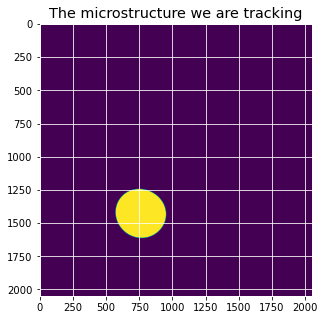
\includegraphics[width=0.9\textwidth]{Pictures/Tracking/Traching_cog.jpeg}
  \caption{COG suited precipitate}
  \label{img:microstrImg}
\end{subfigure}
\begin{subfigure}{.45\textwidth}
  \centering
  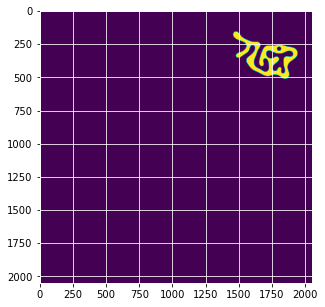
\includegraphics[width=0.9\textwidth]{Pictures/Tracking/Tracking_choosing_ppt.jpeg}
  \caption{Probabilistic model suited precipitate}
  \label{img:MicrostrImg}
\end{subfigure}
\caption{Visualizing Precipitates}
\label{fig:test}
\end{figure}

%%%%%%%%%%%%%%%%%%%%%%%%%%%%%%%%%%%%%%%%%%%
\section{Convexity measures}

\subsection{Definition}
We define Convexity in terms of a number called Convexity number, a probabilistic measure of how convex a binary image is. The convexity number should have the following features for it to be a good indicator of probability \cite{31rahtu2006new}:
\begin{enumerate}
    \item A number lies between (0,1], with a perfectly convex shape having a value of 1
    \item The number increases as the convexity of the image increases
\end{enumerate}

A image is perfectly convex if given any 2 points taken on the image, the line joining the 2 points entirely lies in the image. Analogous to this definition, we define our convexity to measure the likeliness of this line joining 2 points on the image to lie on the image. The convexity measure we calculate is the following:

\textbf{\textit{Given 2 points on the image, what is the probability that a third point in the midpoint of these 2 points lies on the image as well.}}

We simplify to account only for the midpoint since the midpoint lying on the line is often a good indicator of the whole line being on the line, and just calculating the midpoint saves us the computation time of calculating all the points in the line. The measure can thus be formally written as the following:


For points $p_i$ in the binary image space $I$ and $m_{ij}$ being the midpoints of 2 points $p_i$ and $p_j$ , we calculate:

\begin{equation}
    P_{convexity} = P(m_{ij} = 1 | p_i = 1 \cap p_j = 1 )
\end{equation}
\myequations{Convexity formulation}


This convexity measure is extremely difficult to compute, and theorems like the Convolution theorem we applied while calculating auto-correlations fail because of the presence of the extra midpoint term in the expression. We thus calculate this quantity by using Monte Carlo techniques.

% Add image of a concave and a convex precipitate here for understanding
\begin{figure}[H]
\centering
\begin{subfigure}{.45\textwidth}
  \centering
  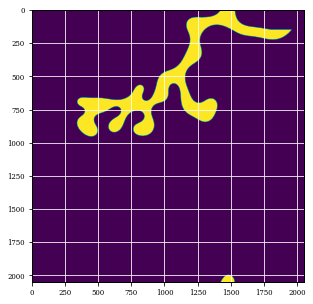
\includegraphics[width=0.9\textwidth]{Pictures/MSFeatures/ExampleConcavePPT.png}
  \caption{Concave Precipitate}
  \label{img:microstrImg}
\end{subfigure}
\begin{subfigure}{.45\textwidth}
  \centering
  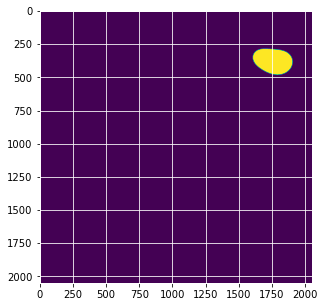
\includegraphics[width=0.9\textwidth]{Pictures/MSFeatures/ExampleConvexPPT.png}
  \caption{Convex Precipitate}
  \label{img:microstrImg}
\end{subfigure}
\caption{Visualizing Concave and Convex shapes}
\label{fig:test}
\end{figure}



\subsection{Monte Carlo method}
Since calculating the exact probability measure is too computationally expensive, we use a Monte Carlo method to sample points from the image and calculate the probability measure. We run the simulation till the probability value converges, which we notice generally happens after 30,000 sampled points for 2000*2000 resolution images.

The formulation of the method is simple. We randomly select 2 points on the image which lie on the object. We then find the point in the middle of the line joining these 2 points, and check whether this point also lies in the object. The net probability measure we calculate then becomes:

\begin{equation}
    P_{convexity} = \frac{\textit{No of midpoints on object}}{\textit{Number of pairs of points chosen on object}}
\end{equation}
\myequations{Monte Carlo definition of convexity}


\subsection{Testing convexity on precipitate growth}
We track 2 precipitates in the spinodal regime who can be observed to be moving towards convexity and test if our convexity measure in increasing in time and finally constant at 1 when the precipitate is perfectly convex. The 2 precipitates perfectly followed our hypothesis, which can be seen in the curves below. 

%% ADD 2 precipitate growth and increase curve
\begin{figure}[H]
\centering
\begin{subfigure}{.32\textwidth}
  \centering
  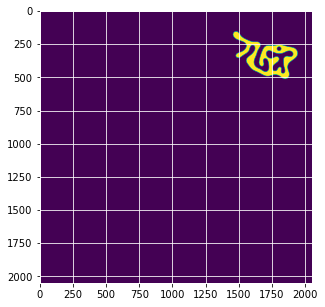
\includegraphics[width=0.9\textwidth]{Pictures/MSFeatures/ConvexMSStart.png}
  \label{img:microstrImg}
\end{subfigure}
\begin{subfigure}{.32\textwidth}
  \centering
  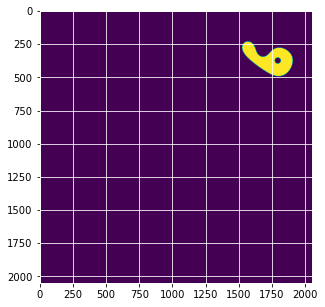
\includegraphics[width=0.9\textwidth]{Pictures/MSFeatures/ConvexMSMiddle.png}
  \label{img:microstrImg}
\end{subfigure}
\begin{subfigure}{.32\textwidth}
  \centering
  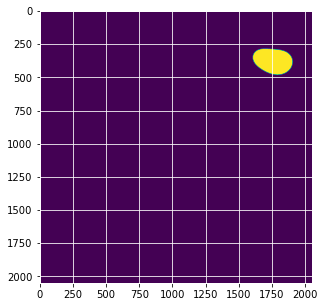
\includegraphics[width=0.9\textwidth]{Pictures/MSFeatures/ConvexMSEnd.png}
  \label{img:microstrImg}
\end{subfigure}
\begin{subfigure}{.5\textwidth}
  \centering
  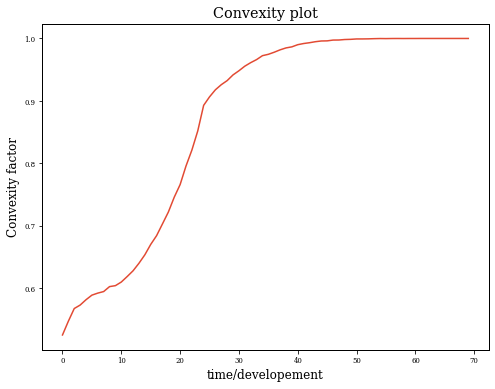
\includegraphics[width=0.9\textwidth]{Pictures/MSFeatures/IsoGrainConvexity.png}
  \label{img:microstrImg}
\end{subfigure}
\caption{Visualizing Convexity Number with Precipitate Growth}
\label{fig:test}
\end{figure}

\subsection{Convexity for complete microstructural images}
Since up until now we have talked only about convexity of individual precipitates, it only makes sense to define convexity in a form to quantify complete microstructural evolution with multiple precipitates. The traditional form of convexity that we define in the earlier section fails when we apply it to more than 1 precipitate in an image, and thus we require a new transformed form of convexity. 

We call this form of convexity \textbf{Short Range Averaged Convexity}. Rather than do the Monte Carlo random point sampling on the entire image, we break the image down into N$*$N smaller images, calculate the convexity for each of these smaller images(called Short Range Convexity), and report the average convexity of these smaller bits. This convexity can be imagined as a measure to ascertain at what length scale the microstructure is locally convex in. The flowchart describing the steps followed is as follows:

\usetikzlibrary{shapes.geometric, arrows}
\tikzstyle{process} = [rectangle, minimum width=3cm, minimum height=1cm, text centered, draw=black]
\tikzstyle{arrow} = [thick,->,>=stealth]
\begin{center}
\begin{tikzpicture}[node distance=2cm]
\node (start) [process] {Load microstructure image};
\node (in1) [process, below of=start] {Divide image into N*N tiles (eg. 4*4)};
\node (in2) [process, below of=in1] {Calculate the convexity of each tile(eg. 16 tiles)};
\node (in3) [process, below of=in2] {Report mean of convexity from all tiles};
\draw [arrow] (start) -- (in1);
\draw [arrow] (in1) -- (in2);
\draw [arrow] (in2) -- (in3);
\end{tikzpicture}
\end{center}

The Short Range Average Convexity values of a developing microstructure showed a steadily increasing value when using a N=4, ie. using 16 tiles. The microstructural evolution and the convexity values are shown below. We can see the steady increase in convexity values clearly with evolution, which verifies our model perfectly.

%% Add the images for micro growth and convexity short range
\begin{figure}[H]
\centering
\begin{subfigure}{.32\textwidth}
  \centering
  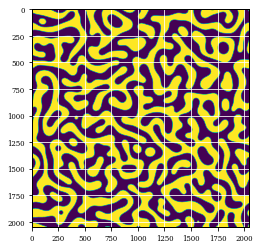
\includegraphics[width=0.9\textwidth]{Pictures/MSFeatures/ConvexMicroEvolStart.png}
  \label{img:microstrImg}
  \caption{time = $t_1$}
\end{subfigure}
\begin{subfigure}{.32\textwidth}
  \centering
  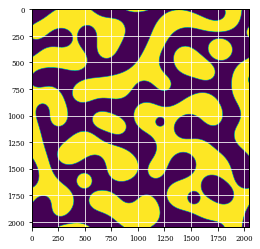
\includegraphics[width=0.9\textwidth]{Pictures/MSFeatures/ConvexMicroExalMiddle.png}
  \label{img:microstrImg}
  \caption{time = $t_2$}
\end{subfigure}
\begin{subfigure}{.32\textwidth}
  \centering
  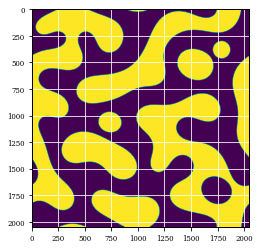
\includegraphics[width=0.9\textwidth]{Pictures/MSFeatures/ConvexMicroEvalEnd.png}
  \caption{time = $t_3$}
  \label{img:microstrImg}
\end{subfigure}
\begin{subfigure}{.5\textwidth}
  \centering
  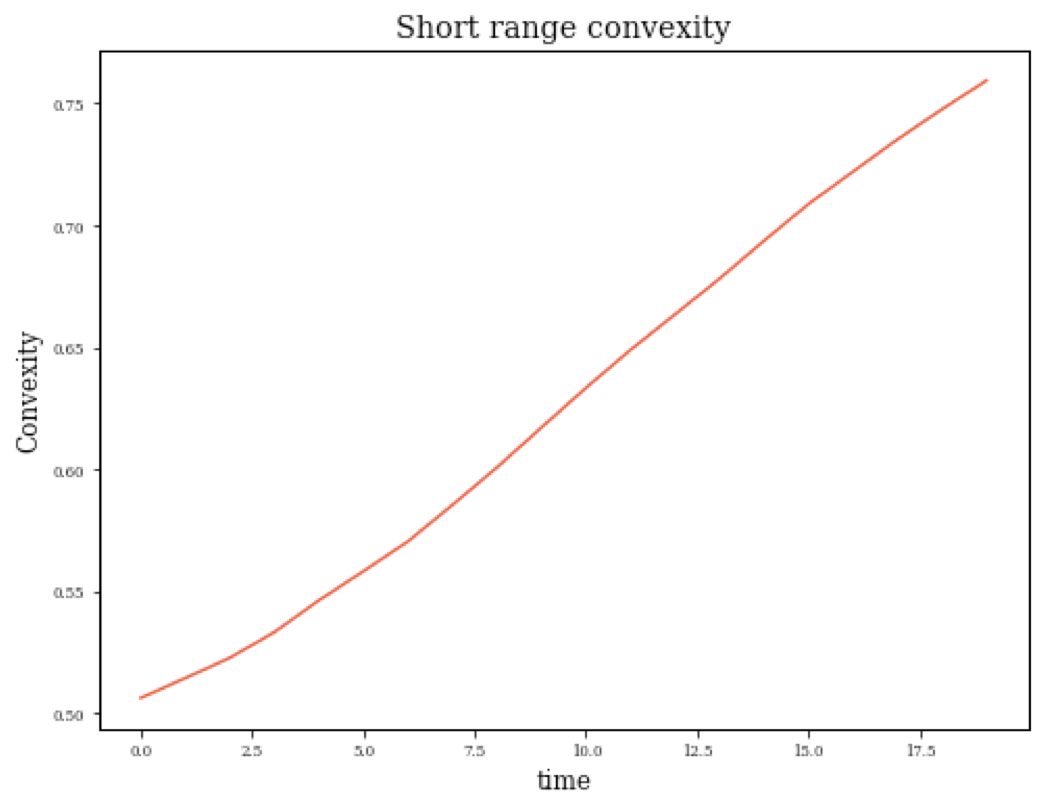
\includegraphics[width=0.9\textwidth]{Pictures/MSFeatures/ShortRangeConvexityIso.png}
  \label{img:microstrImg}
\end{subfigure}
\caption{Convexity number change with Microstructure Evolution ($t_3>t_2>t_1$)}
\label{fig:test}
\end{figure}

\subsection{Calculating Short Range Averaged Convexity using different box sizes}
Since our convexity measures for Short Range Averaged Convexity depends on the number of bits we divide the image into, it becomes imperative to statistically describe the significance of smaller or larger box sizes. Intuitively, smaller box sizes(breaking image into more parts) should lead to higher convexity values for any microstructure, since a microstructure generally tries to obtain perfect convexity along smaller regions first, and then through agglomeration or growth, becomes larger and convex on bigger length scales. 

We do this experiment on Hexagonal microstructures of 3 compositions, 0.3, 0.4 and 0.5, and vary the number of parts we break the image into in the increasing power of 2. That is, we check the convexity values for 2x2, 4x4, 8x8 and 16x16 boxes. The results from the experiment are show below.

\begin{figure}[H]
\centering
\begin{subfigure}{.45\textwidth}
  \centering
  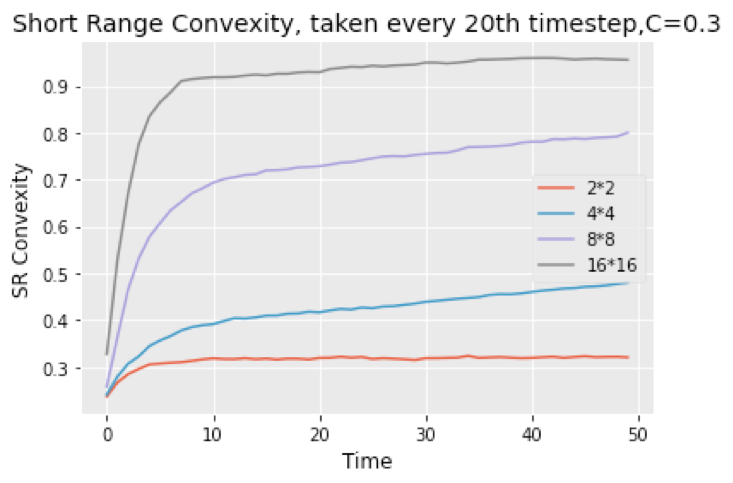
\includegraphics[width=0.9\textwidth]{Pictures/MSFeatures/shac_0.3_24816.png}
  \label{img:microstrImg}
\end{subfigure}
\begin{subfigure}{.45\textwidth}
  \centering
  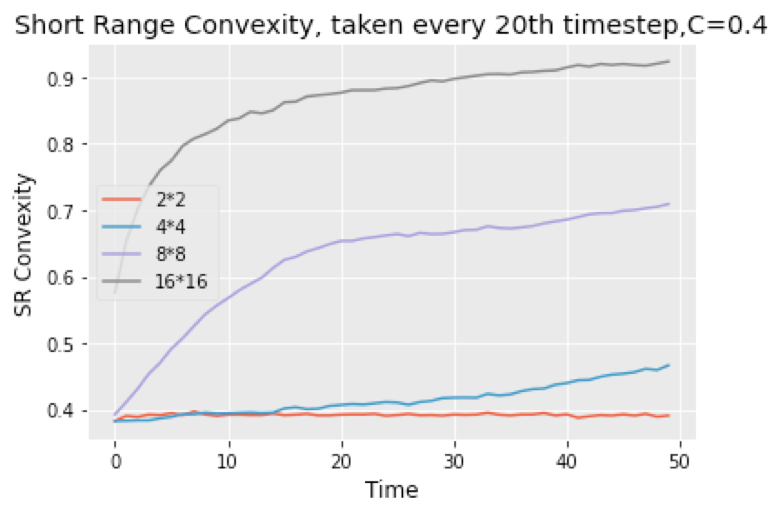
\includegraphics[width=0.9\textwidth]{Pictures/MSFeatures/shac_04_24816.png}
  \label{img:microstrImg}
\end{subfigure}
\begin{subfigure}{.45\textwidth}
  \centering
  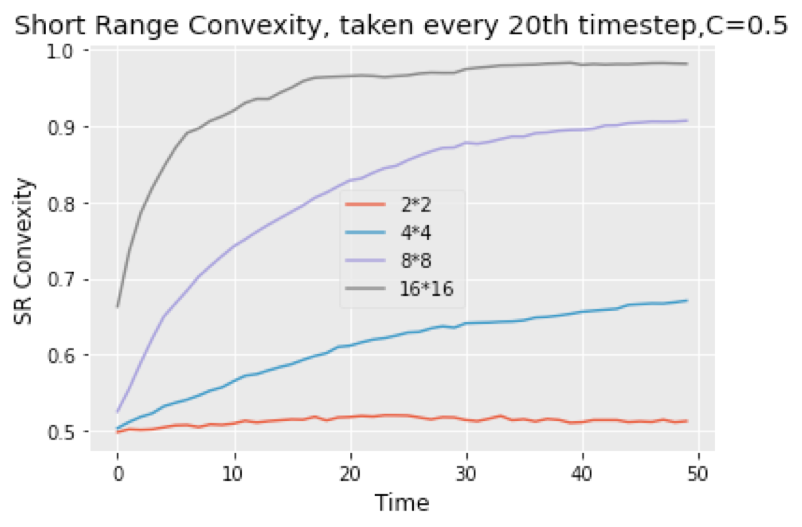
\includegraphics[width=0.9\textwidth]{Pictures/MSFeatures/shac_05_24816.png}
  \label{img:microstrImg}
\end{subfigure}
\caption{Convexity change with different image divisions}
\label{fig:test}
\end{figure}

The plots above illustrate that the more divisions you make(and decrease the individual box sizes), more rapid is the Short Range Averaged Convexity rise. Furthermore, after certain time-steps of microstructural evolution, the higher-division convexity's converge to values close to one. This implies that microstructures develop in a way such that the convexity values increase and asymptotically converge to 1.



%%%%%%%%%%%%%%%%%%%%%%%%%%%%%%%%%%%%%%%%%%%
\chapter{Results and Discussion}
This chapter is divided into 3 parts for easier understanding. 

In the first section (Section 4.1) we use some of the tools and measures discussed in the previous chapter to analyse some sample microstructures and derive conclusions based on these results. The inferences derived from this section will clarify how the outputs from the algorithms in Chapter 3 need to be understood. 

In the second section (Section 4.2), we compare the macroscopic properties of the Isotropic, Cubic and Hexagonal microstructures across time, and identify key distinguishing features between these microstructures. We use the conclusions drawn from Section 4.1 as basis for out comparison.

In the third section (Section 4.3), we test methods of precipitate tracking to identify key events and track precipitate growth. This section is meant to give the reader a sense of the wide range of evolutionary parameters that can be tracked by the clustering and tracking algorithms presented in this report.

\section{Characterisation examples and use cases}
\subsection{Datasets used for comparison}
The Cahn-Hilliard generated microstructures are of three types, the perfectly isotropic, and ones with hexagonal and cubic anisotropy. Each of these were generated for 200,000 time-steps, and every $200^{th}$ image was sampled out for analysis, ie. we had 1000 images to apply statistics to. Upon visual examination of these 1000 images, and noting down the statistical changes observed between different times, we observed that there was little significant change in statistical features between alternate images, ie. images 200 time-steps apart. Thus, to save on computing time we sample only every $30^{th}$  image out of the 1000 images for feature extraction, which gives us enough time-series information to draw conclusions from, since within each 30 continuous images, the statistical difference is insignificant. 


\subsection{2-Point Correlations}
The 2-Point correlations are calculated as explained in Chapter 3. We visualize the precipitate cross-correlation and auto-correlation heat map, and also calculate these metrics on a distance scale, ie. calculating the values on a radial scale by averaging the probability along a thin circular ring. Furthermore, we extend this analysis to capture angular features along particular angular sectors, to capture anisotropy. These 3 use cases are presented in the subsections ahead.

\subsubsection{Using 2-Point correlation to compare anisotropy}
The auto-correlations represented as a probability heat-map is calculated for microstructures at different stages of their evolution. The points on the vector space(with the centre of the image as the origin) with color higher up on the color-bar represent higher probability of occurrence of the particular local state. For instance, at the centre(vector (0,0)), the probability will always be exactly equal to the probability of finding the local state(ie. 0.3 if we calculate auto-correlations for composition 0.3). Furthermore, we can generally observe rings of higher and lower probability close to the origin, which are good indicators of the periodicity in the microstructures.  

For instance, in the below figures, you can observe the auto and cross correlations calculated for the isotropic case of precipitate phase composition 0.5, which demonstrate the properties mentioned in the previous paragraph. We can clearly observe that the auto-correlations and cross-correlations for the isotropic microstructures have no anisotropy, and are perfectly spherically contoured as shown below. The high probability spherical rings are also perfectly visible around the centre, showing the approximate judgement of precipitate sizes. 

% Add autocorr and cross corr for isotropic
\begin{figure}[H]
\centering
\begin{subfigure}{.32\textwidth}
  \centering
  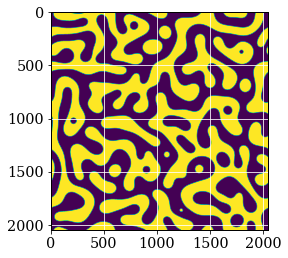
\includegraphics[width=0.9\textwidth]{Pictures/MSFeatures/CorrIsoImage.png}
  \caption{Image, Isotropic C=0.5}
  \label{img:microstrImg}
\end{subfigure}
\begin{subfigure}{.32\textwidth}
  \centering
  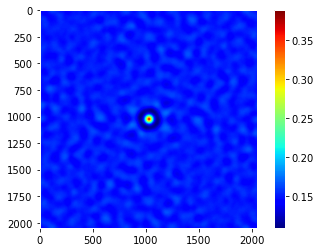
\includegraphics[width=0.9\textwidth]{Pictures/MSFeatures/CorrImageAuto.png}
  \caption{Auto-correlation}
  \label{img:microstrImg}
\end{subfigure}
\begin{subfigure}{.32\textwidth}
  \centering
  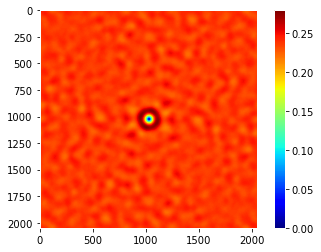
\includegraphics[width=0.9\textwidth]{Pictures/MSFeatures/CorrImageCross.png}
  \caption{Cross-correlation}
  \label{img:microstrImg}
\end{subfigure}
\caption{Visualizing Correlation for Isotropic Microstructures}
\label{fig:test}
\end{figure}

For the hexagonal microstructure of composition of precipitate phase 0.5, visualizing the probability correlation heat-map gives expected results. For the hexagonal case, we can clearly see the anisotropy in the precipitate distribution in the figures below in the form of the hexagons of high and low probability around the centre, which adds credence to our formulation. 

% Add autocorr and cross corr for hexa
\begin{figure}[H]
\centering
\begin{subfigure}{.32\textwidth}
  \centering
  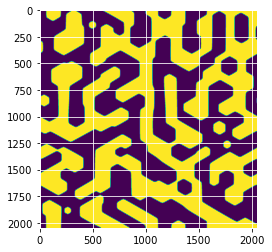
\includegraphics[width=0.9\textwidth]{Pictures/MSFeatures/CorrHexaImage.png}
  \caption{Image, Hexagonal C=0.5}
  \label{img:microstrImg}
\end{subfigure}
\begin{subfigure}{.32\textwidth}
  \centering
  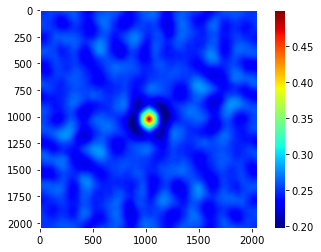
\includegraphics[width=0.9\textwidth]{Pictures/MSFeatures/CorrHexaAuto.png}
  \caption{Auto-correlation}
  \label{img:microstrImg}
\end{subfigure}
\begin{subfigure}{.32\textwidth}
  \centering
  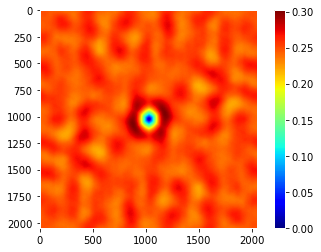
\includegraphics[width=0.9\textwidth]{Pictures/MSFeatures/CorrHexaCross.png}
  \caption{Cross-correlation}
  \label{img:microstrImg}
\end{subfigure}
\caption{Visualizing Correlation for Hexagonal Microstructures}
\label{fig:test}
\end{figure}
By using these correlation heatmaps, we can get a fair idea about the anisotropy shape/directions, and also judge the particle sizes by looking at the sized of the rings around the centre. Thus, these heatmaps capture important macroscopic features from the binary microstructure images. 


\subsubsection{Using 2-Point Radial Correlations to study microstructure evolution}
\label{radialCorrelationDerivation}

Although the correlation heatmaps give us significant information about the anisotropy and approximate sizes of the precipitates, these are not easily numerically quantifiable through heatmaps. Thus, we plot the radial correlations($S_2(r)$) as a measure, derived directly from the probability heatmaps above, which can quantify the understanding of the particle sizes. 

We calculate the radial auto-correlation as the auto-correlation taken and averaged at a particular radial distance. This is calculated by simply taking a correlation plot, and finding the average probability at thin rings of radius $r$ around the centre. This way, we can capture more easily the particle distribution at a radial distance $r$ from the origin. This plot gives us important information about the probability distribution of precipitates, and can help us identify the particle size and inter particle distance of a microstructure. 

The x-coordinate represents the radial distance from the origin, while the y axis represents the probability of finding the same local state(in our auto-correlations case - the precipitate) at that radial distance. The first x-coordinate minima of the radial auto-correlation curve corresponds to the precipitate size(ie. where the likelihood of finding the precipitate is lowest), while the first maxima after the origin is an indication of the inter-particle distance(ie. where the likelyhood of finding another precipitate is highest again).

These 2 measures can be plotted across time to study precipitate size growth and distribution in microstructural evolution. As we can observe in the figures below for the Hexagonal Microstructures as an example, the plots are largely oscillatory, implying subsequent higher and lower probability regions of finding precipitate in a microstructure, which holds well with our microstructural image. Furthermore, as we make this plot at increasing intervals of time, the curve moves towards the rights, ie. the precipitate size and inter-particle distance both increase as the microstructure evolves, which also holds true with our images.

Additionally, the difference in probability values of precipitates at different compositions in the figure below clearly shows us how composition changes affect particle sizes and distances.

% Add image for radial autocorr and crosscorr one each
\begin{figure}[H]
\centering
\begin{subfigure}{.9\textwidth}
  \centering
  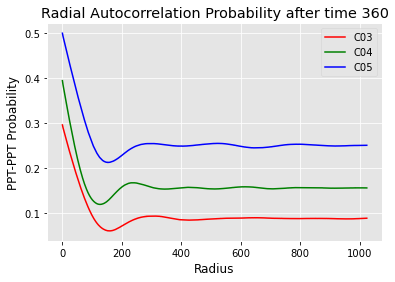
\includegraphics[width=0.9\textwidth]{Pictures/MSFeatures/RadialCorrExample.png}
  \label{img:microstrImg}
\end{subfigure}
\caption{Plotting Radial Auto Correlations}
\label{fig:test}
\end{figure}

%radial change with time plotted
\begin{figure}[H]
\centering
\begin{subfigure}{.48\textwidth}
  \centering
  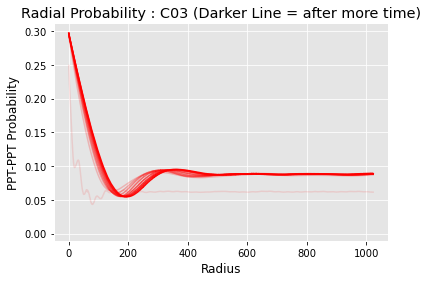
\includegraphics[width=0.95\textwidth]{Pictures/MSFeatures/RadC03MovRight.png}
  \label{img:microstrImg}
\end{subfigure}
\begin{subfigure}{.48\textwidth}
  \centering
  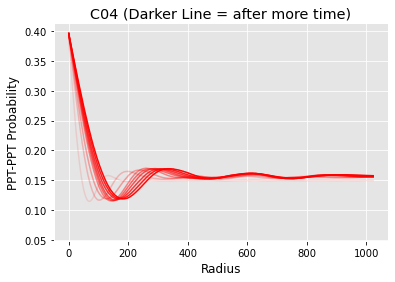
\includegraphics[width=0.95\textwidth]{Pictures/MSFeatures/RadC04MovRight.png}
  \label{img:microstrImg}
\end{subfigure}
\begin{subfigure}{.48\textwidth}
  \centering
  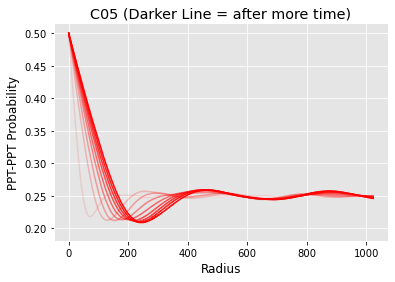
\includegraphics[width=0.95\textwidth]{Pictures/MSFeatures/RadC05MovRight.png}
  \label{img:microstrImg}
\end{subfigure}

\caption{Plotting radial auto-correlations vs time}
\label{fig:unexplainablePlot}
\end{figure}

The radial auto-correlation change with time gives us a good indication of precipitate growth as the we can clearly see the radial curve spread out/decrease in frequency as the microstructure evolves.


\subsubsection{Contrasting directions of anisotropy with correlations along directions}
In cases of anisotropy, it becomes imperative to establish precipitate growth in different directions, as a single radial correlation does not give us information about the anisotropy in the system. This can be done simply by plotting the radial correlation only between certain angles ie. sectors to compare the evolution along these angles. That is, rather than calculating the mean probability over a ring around the origin, we calculate the mean along an angular arc on the ring. 

This can be done in 2 ways, comparing growth/size along a particular direction to the average growth/size, or comparing distributions between directions of anisotropy. This itself becomes a test for anisotropy, as a perfectly isotropic microstructure will show identical radial behavior along all angles and directions for small radii in the neighbourhood.

% Plot of radial vs 3060 degree
\begin{figure}[H]
\centering
\begin{subfigure}{.49\textwidth}
  \centering
  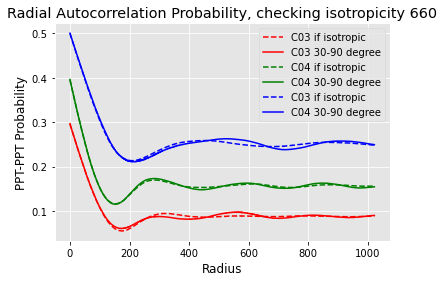
\includegraphics[width=0.95\textwidth]{Pictures/MSFeatures/ShowingAnisotropyAngle.png}
  \label{img:microstrImg}
  \caption{Comparing radial and angular correlation as an anisotropy test}
\end{subfigure}
\begin{subfigure}{.49\textwidth}
  \centering
  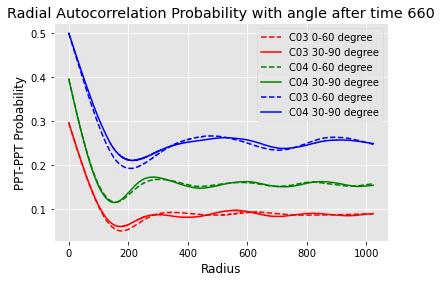
\includegraphics[width=0.95\textwidth]{Pictures/MSFeatures/RadialCorr306090Comparison.png}
  \caption{Comparing 2 different angles of growth}
  \label{img:microstrImg}
\end{subfigure}

\caption{Comparing directional growth}
\label{fig:test}
\end{figure}

We can also compare angles of growth to understand in which directions the anisotropy is prominent. We compare 2 sectors of 60 degrees each in the curves above.

\subsection{Using Clustering algorithms for precipitate counting and size estimation}

\begin{figure}[H]
\centering
\begin{subfigure}{.45\textwidth}
  \centering
  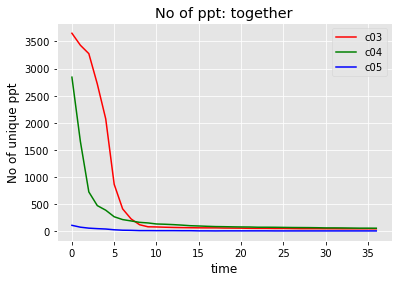
\includegraphics[width=0.9\textwidth]{Pictures/PPTCount/ParticleSizeDist.png}
  \caption{Plotting number of particles}
  \label{img:microstrImg}
\end{subfigure}
\begin{subfigure}{.45\textwidth}
  \centering
  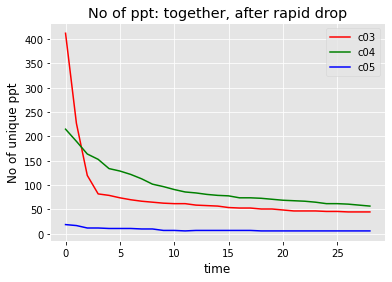
\includegraphics[width=0.9\textwidth]{Pictures/PPTCount/ParticleSizeDistAfterDrop.png}
  \caption{Close up view of particle count}
  \label{img:microstrImg}
\end{subfigure}
\caption{Particle Counting with time}
\label{fig:test22}
\end{figure}
Since we have implemented the Hoshen-Kopelman algorithms to segment individual clusters of precipitates, we can also easily capture the macroscopic properties like the number of precipitates, average precipitate size and standard deviation across both composition and time. These features are more versatile in the initial time periods of microstructural development, and asymptotically converge as the microstructure grows to larger precipitates. 

For instance, the figure below shows the mean, standard deviation and precipitate count comparison of Hexagonal microstructures of precipitate phase composition 0.3 and 0.4 across time. We also plot the total precipitate area in the figure below, which is an indicator of how quickly complete phase separation takes place form the precipitate to the matrix phase(as indicated by the asymptote in the figure).

\begin{figure}[H]
\centering
\begin{subfigure}{.45\textwidth}
  \centering
  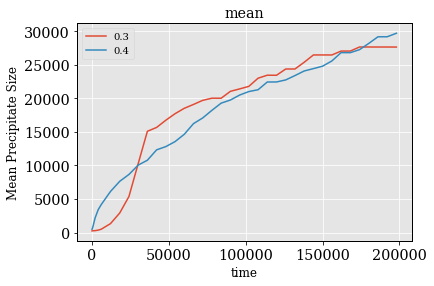
\includegraphics[width=0.9\textwidth]{Pictures/MSFeatures/mean_size.png}
  \caption{Mean}
  \label{img:microstrImg}
\end{subfigure}
\begin{subfigure}{.45\textwidth}
  \centering
  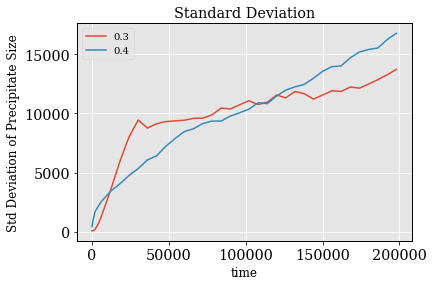
\includegraphics[width=0.9\textwidth]{Pictures/MSFeatures/std_size.png}
  \caption{Std. Deviation}
  \label{img:microstrImg}
\end{subfigure}
\begin{subfigure}{.45\textwidth}
  \centering
  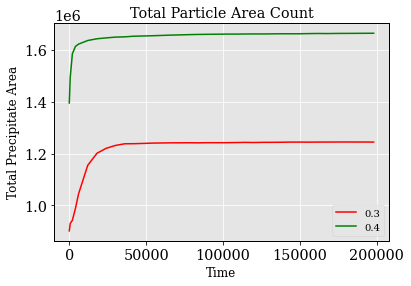
\includegraphics[width=0.9\textwidth]{Pictures/MSFeatures/total_size.png}
  \caption{Total Precipitate Area}
  \label{img:microstrImg}
\end{subfigure}
\caption{Precipitate Size statistics}
\label{fig:test22}
\end{figure}



Furthermore, we can also try and fit the precipitate areas into an area and log area distribution to better understand the precipitate size distribution by plotting histograms. The histograms are only useful with large number of precipitates in the image, and show prominence within the initial stages of the microstructure development. The typical histograms of really early stage microstructures look like the figure below.

\begin{figure}[H]
\centering
\begin{subfigure}{.9\textwidth}
  \centering
  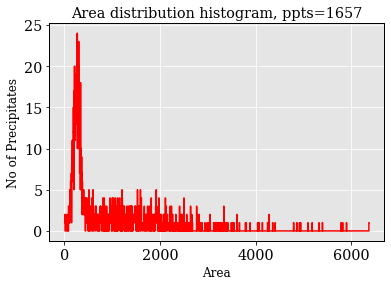
\includegraphics[width=0.9\textwidth]{Pictures/MSFeatures/Area_hist.png}
  \caption{Precipitate Size Distribution}
  \label{img:microstrImg}
\end{subfigure}
\label{fig:test22}
\end{figure}

% What is interesting to note here is that when we compare the microstructural evolution of composition 0.3 and 0.4, the particle size remains almost the same in both cases, which sounds non-intuitive since C0.4 has a greater concentration of the component controlling precipitate formation. The first curve shows that as the microstructure evolves, the number of precipitates reduce, which shows that growth has taken place and smaller precipitates have either vanished or agglomerated with the bigger precipitates. The second figure, which is a zoomed-in image of the first plot (to the right end of the time series data), shows that the number of precipitates in the 0.4 composition are more than the ones at 0.3. This means that even though the average precipitate size remains almost identical in 0.4 to 0.3, the number of precipitates with that size have increased. This means that when we go from C0.3 to C0.4, the additional composition is used in forming more precipitates rather than growing the present precipitates to larger sizes. This explains the ambiguity we saw in Section 7.2 and Fig. \ref{fig:unexplainablePlot}.

\section{Comparison between Isotropic, Hexagonal and Cubic Microstructures}
\subsection{Auto-Correlation Heat-maps}
The Auto-Correlation heatmaps of the three microstructure types can give us clear information about the type of anisotropy and the precipitate size. The figure below illustrates this behaviour for all three types of microstructure(Isotropic, Hexagonal and Cubic). The image and the auto-correlation corresponding to that image are shown below.

\begin{figure}[H]
\centering
\begin{subfigure}{.45\textwidth}
  \centering
  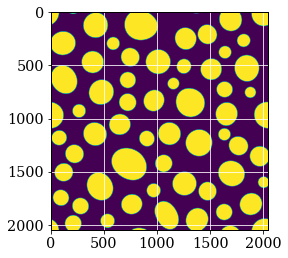
\includegraphics[width=0.9\textwidth]{Pictures/Comparison/iso_img.png}
  \caption{Isotropic Image}
  \label{img:microstrImg}
\end{subfigure}
\begin{subfigure}{.5\textwidth}
  \centering
  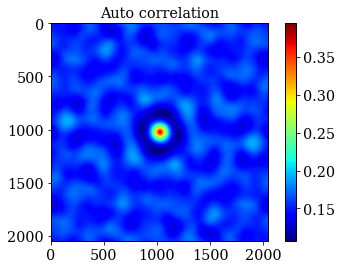
\includegraphics[width=0.9\textwidth]{Pictures/Comparison/iso_heatmap.png}
  \caption{Isotropic Auto-correlation}
  \label{img:microstrImg}
\end{subfigure}

\begin{subfigure}{.45\textwidth}
  \centering
  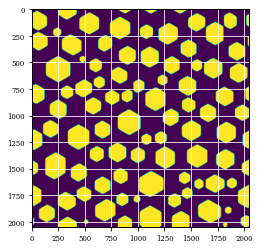
\includegraphics[width=0.9\textwidth]{Pictures/Comparison/hexa_img.png}
  \caption{Hexagonal Image}
  \label{img:microstrImg}
\end{subfigure}
\begin{subfigure}{.5\textwidth}
  \centering
  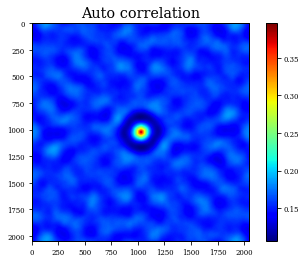
\includegraphics[width=0.9\textwidth]{Pictures/Comparison/hexa_heatmap.png}
  \caption{Hexagonal Auto-correlation}
  \label{img:microstrImg}
\end{subfigure}

\begin{subfigure}{.45\textwidth}
  \centering
  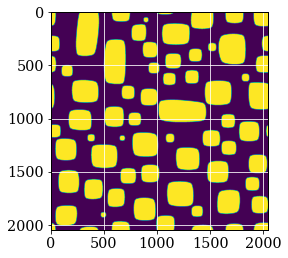
\includegraphics[width=0.9\textwidth]{Pictures/Comparison/cub_img.png}
  \caption{Cubic Image}
  \label{img:microstrImg}
\end{subfigure}
\begin{subfigure}{.5\textwidth}
  \centering
  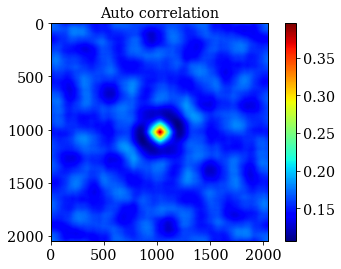
\includegraphics[width=0.9\textwidth]{Pictures/Comparison/cubic_heatmap.png}
  \caption{Cubic Auto-correlation}
  \label{img:microstrImg}
\end{subfigure}
\caption{Comparison of Auto-correlation Heatmaps}
\label{fig:test22}
\end{figure}

The striking feature which is easily noticeable is the probability distribution along the shapes of the original image, that is, given the auto-correlations of an image, we can easily identify the underlying shape anisotropy in the microstructure. The plots below are a zoomed in and high contrast image of Fig 4.9.

\begin{figure}[H]
\centering
\begin{subfigure}{.32\textwidth}
  \centering
  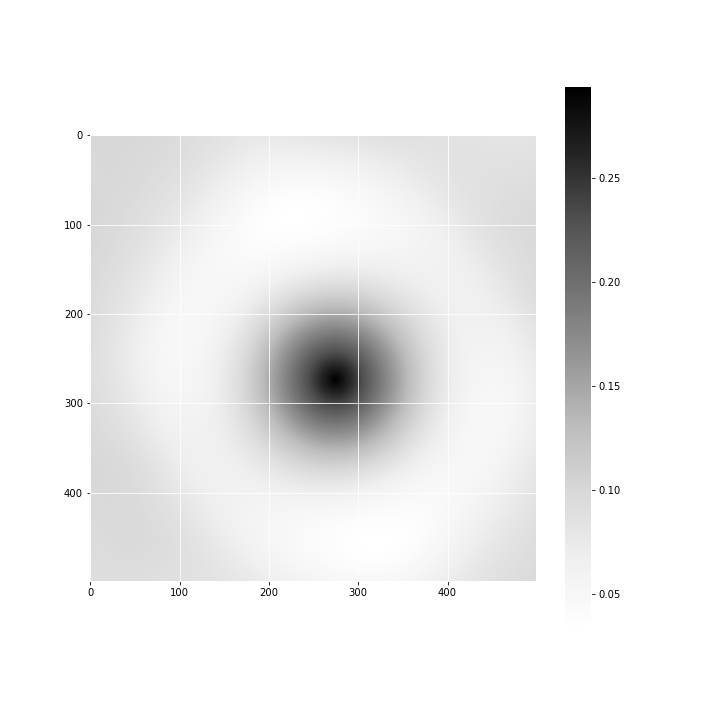
\includegraphics[width=0.9\textwidth]{Pictures/images9/iso_image_03_560.png}
  \label{img:microstrImg}
\end{subfigure}
\begin{subfigure}{.32\textwidth}
  \centering
  \includegraphics[width=0.9\textwidth]{Pictures/images9/iso_image_04_560.png}
  \label{img:microstrImg}
\end{subfigure}
\begin{subfigure}{.32\textwidth}
  \centering
  \includegraphics[width=0.9\textwidth]{Pictures/images9/iso_image_05_560.png}
  \label{img:microstrImg}
\end{subfigure}

\begin{subfigure}{.32\textwidth}
  \centering
  \includegraphics[width=0.9\textwidth]{Pictures/images9/hex_image_03_560.png}
  \label{img:microstrImg}
\end{subfigure}
\begin{subfigure}{.32\textwidth}
  \centering
  \includegraphics[width=0.9\textwidth]{Pictures/images9/hex_image_04_560.png}
  \label{img:microstrImg}
\end{subfigure}
\begin{subfigure}{.32\textwidth}
  \centering
  \includegraphics[width=0.9\textwidth]{Pictures/images9/hex_image_05_560.png}
  \label{img:microstrImg}
\end{subfigure}

\begin{subfigure}{.32\textwidth}
  \centering
  \includegraphics[width=0.9\textwidth]{Pictures/images9/cub_image_03_560.png}
  \label{img:microstrImg}
\end{subfigure}
\begin{subfigure}{.32\textwidth}
  \centering
  \includegraphics[width=0.9\textwidth]{Pictures/images9/cub_image_04_560.png}
  \label{img:microstrImg}
\end{subfigure}
\begin{subfigure}{.32\textwidth}
  \centering
  \includegraphics[width=0.9\textwidth]{Pictures/images9/cub_image_05_560.png}
  \label{img:microstrImg}
\end{subfigure}
\caption{Left to Right: Increasing Composition, Top to bottom: Isotropic, Hexagonal and Cubic }
\label{fig:big9fig}
\end{figure}


We can also compare auto-correlations at different time of evolution. The figures below Fig \ref{fig:big9fig} show how the auto-correlations vary for hexagonal microstructures of precipitate phase composition 0.4 during evolution.

\begin{figure}[H]
\centering
\begin{subfigure}{.32\textwidth}
  \centering
  \includegraphics[width=0.9\textwidth]{Pictures/images9/hexTime/hexa_image_04_100.png}
  \caption{t=100}
  \label{img:microstrImg}
\end{subfigure}
\begin{subfigure}{.32\textwidth}
  \centering
  \includegraphics[width=0.9\textwidth]{Pictures/images9/hexTime/hex_image_04_560.png}
  \caption{t=500}
  \label{img:microstrImg}
\end{subfigure}
\begin{subfigure}{.32\textwidth}
  \centering
  \includegraphics[width=0.9\textwidth]{Pictures/images9/hexTime/hex_image_04_960.png}
  \caption{t=1000}
  \label{img:microstrImg}
\end{subfigure}
\caption{Auto-correlation variation with time for Hexagonal Microstructure with C=0.4}
\label{fig:3HexaTime}
\end{figure}

It is fairly visible in Fig \ref{fig:3HexaTime} that as time of evolution increases, the size of the precipitates as indicated by the size of the dark 'high probability' region also increases. The next Section \ref{radialCorrelation} discusses the quantification of this region.





\subsection{Radial Correlations}
\label{radialCorrelation}
We calculate the Radial Auto-Correlations (as explained in Section  \ref{radialCorrelationDerivation} ) for the three microstructures, which give us easily quantifiable information about the precipitate sizes and distribution. We make the plots to compare how the radial auto-correlation changes based on composition and anisotropy. 

The plots below compare the radial auto-correlations for the 3 types of microstructure(at a composition of 0.4) at 4 different time-steps, initial stage of development, middle phases and towards the end. We can see quite clearly that the radial distribution of different anisotropic microstructures vary significantly in the initial stages, where there are more precipitates, and gradually becomes similar as the microstructures evolve.

\begin{figure}[H]
\centering
\begin{subfigure}{.45\textwidth}
  \centering
  \includegraphics[width=0.9\textwidth]{Pictures/Comparison/Radial Auto comparison/rad_18000.png}
  \caption{Start of evolution}
  \label{img:microstrImg}
\end{subfigure}
\begin{subfigure}{.45\textwidth}
  \centering
  \includegraphics[width=0.9\textwidth]{Pictures/Comparison/Radial Auto comparison/rad_90000.png}
  \caption{Middle Stage 1}
  \label{img:microstrImg}
\end{subfigure}

\begin{subfigure}{.45\textwidth}
  \centering
  \includegraphics[width=0.9\textwidth]{Pictures/Comparison/Radial Auto comparison/rad_120000.png}
  \caption{Middle Stage 2}
  \label{img:microstrImg}
\end{subfigure}
\begin{subfigure}{.45\textwidth}
  \centering
  \includegraphics[width=0.9\textwidth]{Pictures/Comparison/Radial Auto comparison/rad_19200.png}
  \caption{Towards end of evolution}
  \label{img:microstrImg}
\end{subfigure}
\caption{Comparison of Radial Auto-correlations with time between Isotropic, Hexagonal and Cubic for composition of 0.4}
\label{fig:test22}
\end{figure}
Furthermore, if we look at the 3 microstructure types separately, and plot the radial auto-correlations at different compositions, we can see how increasing or decreasing the composition affects the probability distribution of precipitates. The figure below illustrates that as the composition increases, the probability of finding the precipitates in space increases, while the particle size tends to also increase (as demonstrated by the shift of the first minima towards the right). This expected behaviour was followed in the Isotropic and Cubic case, while the Hexagonal microstructures showed some deviation from this behaviour, ie. the average precipitate size at similar time does not increase with increasing composition.

\begin{figure}[H]
\centering
\begin{subfigure}{.45\textwidth}
  \centering
  \includegraphics[width=0.9\textwidth]{Pictures/Comparison/Radial Auto comparison/iso_90k_C345.png}
  \caption{Isotropic}
  \label{img:microstrImg}
\end{subfigure}
\begin{subfigure}{.45\textwidth}
  \centering
  \includegraphics[width=0.9\textwidth]{Pictures/Comparison/Radial Auto comparison/hex_90k_C345.png}
  \caption{Hexagonal}
  \label{img:microstrImg}
\end{subfigure}

\begin{subfigure}{.45\textwidth}
  \centering
  \includegraphics[width=0.9\textwidth]{Pictures/Comparison/Radial Auto comparison/Cub_90k_C345.png}
  \caption{Cubic}
  \label{img:microstrImg}
\end{subfigure}
\caption{Comparison of Radial Auto-correlations between Isotropic, Hexagonal and Cubic with composition}
\label{fig:test22}
\end{figure}

Quite clearly, the Cubic and Isotropic microstructures show the expected behaviour between the compositions of 0.3 and 0.4, that is the probability increases and the first minima(indicator of precipitate size) moves to the right. The hexagonal microstructure shows the probability increase, but the minima at composition 0.4 is to the left of the minima at composition 0.3. This would indicate that the average precipitate size in the composition 0.4 is smaller than the size at composition 0.3. Thus, to study this more closely, we take the Hexagonal microstructures at further finer compositions of 0.3, 0.35, 0.4, 0.41, 0.42, 0.43, 0.45 and 0.5 to see at what composition ranges this behaviour is present. The plots below show the same.

\begin{figure}[H]
\centering
\begin{subfigure}{.45\textwidth}
  \centering
  \includegraphics[width=0.9\textwidth]{Pictures/Comparison/Radial Auto comparison/hex_36k_C3453545.png}
  \caption{Initial Stage}
  \label{img:microstrImg}
\end{subfigure}
\begin{subfigure}{.45\textwidth}
  \centering
  \includegraphics[width=0.9\textwidth]{Pictures/Comparison/Radial Auto comparison/hex_90k_C3453545.png}
  \caption{Middle Stage}
  \label{img:microstrImg}
\end{subfigure}

\begin{subfigure}{.45\textwidth}
  \centering
  \includegraphics[width=0.9\textwidth]{Pictures/Comparison/Radial Auto comparison/hex_168k_C3453545.png}
  \caption{Final Stages}
  \label{img:microstrImg}
\end{subfigure}
\caption{Comparison of Radial Auto-correlations of Hexagonal Microstructure with finer compositions}
\label{fig:test22}
\end{figure}

It's clear that the average precipitate size seems to be decreasing from Composition 0.3 to 0.42, and after 0.42 till the composition of 0.5, the estimate of precipitate size shows increments. Furthermore, if we look closely at the graph at the x coordinate of the first maxima after origin (an indicator of inter-precipitate distance), the inter-precipitate distance seems to have reduced too, which is also counter intuitive since we expect the inter-precipitate distance to increase as precipitates grow. One idea which could explain both these peculiar phenomena is that in the hexagonal case, due to the increase in the number of precipitates, the number of larger precipitates reduce to accommodate many smaller precipitates. That would explain the decrease in the precipitate size and the inter-precipitate distance. We will study and test this hypothesis in the next section(Section \ref{pptSizeStat}).


\subsection{Precipitate Size Statistics}
\label{pptSizeStat}
Let us first look at the mean particle area/size for the 3 Microstructure types(Isotropic, Hexagonal and Cubic) along different compositions. The plots below demonstrate this statistical parameter at 2 different compositions of 0.3 and 0.4. 


\begin{figure}[H]
\centering
\begin{subfigure}{.7\textwidth}
  \centering
  \includegraphics[width=0.9\textwidth]{Pictures/images9/hexTime/meanSizeComparison.png}
  \caption{Mean Precipitate Size with time}
  \label{img:microstrImg}
\end{subfigure}
\caption{Comparison of Mean Precipitate Size of composition 0.3 and 0.4}
\label{fig:test22}
\end{figure}

What is really interesting in the plots above is that the mean precipitate size increases with composition for both cubic and isotropic microstructures, but not for hexagonal microstructures. The mean precipitate size remains nearly equal for both compositions(0.3 and 0.4) in the case of hexagonal microstructures. 

% \begin{figure}[H]
% \centering
% \begin{subfigure}{.45\textwidth}
%   \centering
%   \includegraphics[width=0.9\textwidth]{Pictures/Comparison/Radial Auto comparison/sd_iso.png}
%   \caption{Isotropic}
%   \label{img:microstrImg}
% \end{subfigure}
% \begin{subfigure}{.45\textwidth}
%   \centering
%   \includegraphics[width=0.9\textwidth]{Pictures/Comparison/Radial Auto comparison/sd_hex.png}
%   \caption{Hexagonal}
%   \label{img:microstrImg}
% \end{subfigure}

% \begin{subfigure}{.45\textwidth}
%   \centering
%   \includegraphics[width=0.9\textwidth]{Pictures/Comparison/Radial Auto comparison/sd_cub.png}
%   \caption{Cubic}
%   \label{img:microstrImg}
% \end{subfigure}
% \caption{Comparison of Mean Precipitate Size of composition 0.3 and 0.4}
% \label{fig:test22}
% \end{figure}

So we can conclude that the mean precipitate size does not increase in the hexagonal case significantly between the composition ranges 0.3 to 0.45, but it does in the Isotropic and the Cubic case. This is primarily due to the increase in the number of smaller and similarly sized precipitates. Possible explanations of this phenomena could be due to the constraint in the directions of agglomeration of hexagonal microstructures due to their microscopy.

Finally, another important characteristic to study is the total separation of the precipitate generating phase, that is, to find whether the components are fully separated or not. This can be easily seen when we plot the total area of precipitates, and upon complete separability, this area should be almost constant, or asymptotically constant. Plotting this for the 3 microstructure types gives us the following asymptotic curves.

\begin{figure}[H]
\centering
\begin{subfigure}{.45\textwidth}
  \centering
  \includegraphics[width=0.9\textwidth]{Pictures/Comparison/Radial Auto comparison/tot_iso.png}
  \caption{Isotropic}
  \label{img:microstrImg}
\end{subfigure}
\begin{subfigure}{.45\textwidth}
  \centering
  \includegraphics[width=0.9\textwidth]{Pictures/Comparison/Radial Auto comparison/tot_hex.png}
  \caption{Hexagonal}
  \label{img:microstrImg}
\end{subfigure}

\begin{subfigure}{.45\textwidth}
  \centering
  \includegraphics[width=0.9\textwidth]{Pictures/Comparison/Radial Auto comparison/tot_cub.png}
  \caption{Cubic}
  \label{img:microstrImg}
\end{subfigure}
\caption{Comparing total precipitate area for the the compositions 0.3 and 0.4}
\label{fig:test22}
\end{figure}

We can observe very clearly in the above figures that the total area very quickly grows and asymptotically converges to its maximum value. That is, the initial growth stage in evolving microstructures is driven by dissolution of component from the matrix phase, leading to rapid component separability. The growth after this initial stage becomes slower, something which will be captured in Section \ref{dirGro}.


%%%%%%%%%%%%%%%%%%%%%%%%%%%%%%%%%%%%%%%%%%%
%%%%%%%%%%%%%%%%%%%%%%%%%%%%%%%%%%%%%%%%%%%
\section{Precipitate tracking}

There are specific phenomenon of interest when studying microstructural evolution in precipitates such as directional growth or elongation, agglomeration, inclination and convexity. We take such test cases and demonstrate how our algorithms can identify and track these phenomenon in the subsequent sections. We use isotropic microstructures of compositions 0.3, 0.4 and 0.5 as the test dataset to observe such phenomenon. The features associated with the precipitate being tracked and it's change in time is plotted to demonstrate the above mentioned phenomenon.


\subsection{Directional growth}
\label{dirGro}
Some precipitates grow more in a particular direction non-uniformly, due to the presence of external precipitates or concentration concentrations. Detection of this phenomenon is usually a manual process. We apply our clustering and precipitate tracking algorithms to observe such a precipitate. Figure. \ref{fig:dirGrowImg} shows a precipitate growing in one direction. 

\begin{figure}[H]
\centering
\begin{subfigure}{.45\textwidth}
  \centering
  \includegraphics[width=0.9\textwidth]{Pictures/Growth/1.1.jpeg}
  \caption{$t = t_1$}
  \label{img:microstrImg}
\end{subfigure}
\begin{subfigure}{.45\textwidth}
  \centering
  \includegraphics[width=0.9\textwidth]{Pictures/Growth/1.2.jpeg}
  \caption{$t = t_2$}
  \label{img:microstrImg}
\end{subfigure}
\begin{subfigure}{.45\textwidth}
  \centering
  \includegraphics[width=0.9\textwidth]{Pictures/Growth/1.3.jpeg}
  \caption{$t = t_3$}
  \label{img:microstrImg}
\end{subfigure}
\begin{subfigure}{.45\textwidth}
  \centering
  \includegraphics[width=0.9\textwidth]{Pictures/Growth/1.4.jpeg}
  \caption{$t = t_4$}
  \label{img:microstrImg}
\end{subfigure}

\caption{Directional Growth($t_1<t_2<t_3<t_4$)}
\label{fig:dirGrowImg}
\end{figure}

In bi-directional symmetric growth, although the axis of the precipitate might grow, the COG remains largely steady. The movement of the COG in a particular direction is a indication of how uni-directional the precipitate growth is. Furthermore, directional growth can also be captured by the elongation of the The plots in Fig. \ref{fig:plotDirGrow} capture these features. It is evident that the elongation(captured by sphericity) and the x-coordinate of the precipitate centre see sudden changes due to this directional precipitate growth. 

\begin{figure}[H]
\centering
\begin{subfigure}{.45\textwidth}
  \centering
  \includegraphics[width=0.9\textwidth]{Pictures/Results/1area.jpeg}
  \caption{Area/precipitate growth}
  \label{img:microstrImg}
\end{subfigure}
\begin{subfigure}{.45\textwidth}
  \centering
  \includegraphics[width=0.9\textwidth]{Pictures/Results/1ppts.jpeg}
  \caption{Precipitate count}
  \label{img:microstrImg}
\end{subfigure}
\begin{subfigure}{.45\textwidth}
  \centering
  \includegraphics[width=0.9\textwidth]{Pictures/Results/1lb.jpeg}
  \caption{Studying sphericity}
  \label{img:microstrImg}
\end{subfigure}
\begin{subfigure}{.45\textwidth}
  \centering
  \includegraphics[width=0.9\textwidth]{Pictures/Results/1cogx.jpeg}
  \caption{The x coordinate of COG shows a trough, indicating left sided growth}
  \label{img:microstrImg}
\end{subfigure}
\caption{Precipitate parameter visualization}
\label{fig:plotDirGrow}
\end{figure}

\subsection{Identifying agglomeration}
Many times, 2 precipitates agglomerate to form a single precipitate. Identification of such types of agglomeration is easily noticed by observing the discontinuities in the area of the tracked precipitate. The point of agglomeration sees a significant jump in the precipitate tracked area. Furthermore the elongation ($\frac{l}{b}$) also sees a discontinuity and usually rises rapidly, since agglomeration starts with an elongated structure.
\begin{figure}[H]
\centering
\begin{subfigure}{.24\textwidth}
  \centering
  \includegraphics[width=0.9\textwidth]{Pictures/Growth/2.1.jpeg}
  \label{img:microstrImg}
\end{subfigure}
\begin{subfigure}{.24\textwidth}
  \centering
  \includegraphics[width=0.9\textwidth]{Pictures/Growth/2.2.jpeg}
  \label{img:microstrImg}
\end{subfigure}
\begin{subfigure}{.24\textwidth}
  \centering
  \includegraphics[width=0.9\textwidth]{Pictures/Growth/2.3.jpeg}
  \label{img:microstrImg}
\end{subfigure}
\begin{subfigure}{.24\textwidth}
  \centering
  \includegraphics[width=0.9\textwidth]{Pictures/Growth/2.4.jpeg}
  \label{img:microstrImg}
\end{subfigure}
\label{fig:test}
\end{figure}

We track the microstructure and calculate the area, length/breadth ratio and inclination of the precipitate. It is easily observable that all quantities have a discontinuity in time, especially the area of the precipitate. Thus, given such plots we can identify instances of agglomeration in the microstructure. 

\begin{figure}[H]
\centering
  \begin{subfigure}{.45\textwidth}
  \centering
  \includegraphics[width=0.9\textwidth]{Pictures/Results/2area.jpeg}
  \caption{Discontinuity in area implies start of agglomeration}
  \label{img:microstrImg}
  \end{subfigure}
  \begin{subfigure}{.45\textwidth}
  \centering
  \includegraphics[width=0.9\textwidth]{Pictures/Results/2lb.png}
  \caption{Sudden elongation is presage to future agglomeration}
  \label{img:microstrImg}
  \end{subfigure}
  \begin{subfigure}{.45\textwidth}
  \centering
  \includegraphics[width=0.9\textwidth]{Pictures/Results/2angle.jpeg}
  \caption{Angle of inclination determines direction of agglomeration}
  \label{img:microstrImg}
\end{subfigure}
\caption{Agglomeration: Identification and Tracking}
\label{fig:test}
\end{figure}



\subsection{Precipitate inclination}
The presence of a perfectly spherical precipitate leads to no angle of inclination, so in such cases random noise is usually observed. But more often, due to anisotropy, we generally observe a detectable angle of inclination and elongation ratio. Angle of inclination is calculated by fitting the best ellipse on the precipitate and calculating the inclination with a vertical line, while elongation is defined as the ratio of major and minor axis of the same ellipse. We study one such precipitate growth here, where the inclination and elongation is easily observable.

\begin{figure}[H]
\centering
\begin{subfigure}{.24\textwidth}
  \centering
  \includegraphics[width=0.9\textwidth]{Pictures/Growth/3.1.jpeg}
  \label{img:microstrImg}
\end{subfigure}
\begin{subfigure}{.24\textwidth}
  \centering
  \includegraphics[width=0.9\textwidth]{Pictures/Growth/3.2.jpeg}
  \label{img:microstrImg}
\end{subfigure}
\begin{subfigure}{.24\textwidth}
  \centering
  \includegraphics[width=0.9\textwidth]{Pictures/Growth/3.3.jpeg}
  \label{img:microstrImg}
\end{subfigure}
\begin{subfigure}{.24\textwidth}
  \centering
  \includegraphics[width=0.9\textwidth]{Pictures/Growth/3.4.jpeg}
  \label{img:microstrImg}
\end{subfigure}
\label{fig:test}
\caption{Rapidly evolving precipitate to study elongation }
\end{figure}

\begin{figure}[H]
\centering
\begin{subfigure}{.4\textwidth}
  \centering
  \includegraphics[width=0.8\textwidth]{Pictures/Results/3area.jpeg}
  \caption{We observe a steady precipitate growth}
  \label{img:microstrImg}
\end{subfigure}
\begin{subfigure}{.4\textwidth}
  \centering
  \includegraphics[width=0.8\textwidth]{Pictures/Results/3lb.jpeg}
  \caption{The elongation is easily observable}
  \label{img:microstrImg}
\end{subfigure}
\begin{subfigure}{.4\textwidth}
  \centering
  \includegraphics[width=0.8\textwidth]{Pictures/Results/3theta.jpeg}
  \caption{The angle hovers around the $36^{\circ}$ mark(y-axis)}
  \label{img:microstrImg}
\end{subfigure}
\caption{Inclination is easily observable in the tracked precipitates}
\label{fig:test}
\end{figure}

It is easy to observe that the elongation ratio drops rapidly as the precipitate becomes more spherical. Moreover, the angle of inclination remains constant at ~$36^{\circ}$. Thus, by using these curves, we can estimate the shape change observed in a precipitate during it's evolution.


\chapter{Conclusion}

Data oriented material design is dependent on efficient and useful feature extraction from sources like microstructure images. Algorithms and workflows are needed to simplify extraction of statistical and geometric features, since manual extraction is time consuming. This report aims to identify the features best suited for characterisation and provide robust computationally efficient algorithms for their extraction. By comparing various algorithms and features from literature, and implementing them on computationally generated microstructures, the algorithms and computations required are laid out in this report. The results and plots obtained validate the algorithms, and also provide a visual method of interpreting microstructures. The features extracted quantify the inherent composition distribution, and help draw conclusions from them. 

Spatial probability distributions of local states are crucial to understanding the statistics behind the images, all the while making visual interpretation easier. Comparison of microstructures with varying composition, anisotropy and evolution time based on these distribution provide a visceral understanding of how the evolution takes place. Furthermore, they simplify the analysis of large microstructure data, making their distinct features more prominently noticeable. The algorithms provided are codified and simplified for easier re-utilization and extension to further scientific research, paving the way for the development of more statistical or geometric features based on precipitate tracking or microstructure distributions.

Extraction of useful features is one end of the Process-Structure-Property chain. Modelling of properties from this feature set is the aim of the research field, and is the obvious next step in the research process. This report laid down the foundations of how to extract features, further progress is determined by how these features are used to determine properties. The Structure-property models can be built on computationally simulated data or real world experimental data. The efficiency of the models are determined by how good the training data and feature-set selections are, which this paper aimed to solve. Many methods ranging from regression/classification models, Deep neural nets etc. can be incorporated to build these relations. Additionally, reconstructions based on extracted features can pave the way for building ensembles of microstructure, enabling easier classification of materials only based on microstructure images. 

The next stage of the thesis shall be focused on building these Structure-Property linkages, based on the statistical data extracted by the algorithms presented in this report. 


%%%%%%%%%%%%%%%%%%%%%%%%%%%%%%%%%%%%%%%%%%%%%%
%%%%%%%%%%%%%%%%%%%%%%%%%%%%%%%%%%%%%%%%%%%%%%



\printbibliography



\end{document}          
